% Select one class
%\documentclass{pucthesis}		% For DVI
%\documentclass[pdftex]{pucthesis}	% For pdfLaTeX
%\documentclass[spanish]{pucthesis}		% For DVI, in spanish
\documentclass[pdftex,spanish]{pucthesis}	% For pdfLaTeX, in spanish

%%%%%%%%%%%%%%%%%%%%%%%%%%
%      Nota: si usas español, algunos nombres      %
%      debes cambiarlos manualmente en este     %
%        documento. En teoría, nunca deberías       %
%           modificar el archivo pucthesis.cls              %
%%%%%%%%%%%%%%%%%%%%%%%%%%

%%%%%%%%%
%   Packages	 %
%%%%%%%%%

% Floats
\usepackage{graphicx}
\usepackage{float}
\floatstyle{boxed}
\restylefloat{figure}
\IfFileExists{subfigure.sty}{\usepackage{subfigure}}{}  % no está en el TeX Live local; en Overleaf sí
\usepackage{color}

% Math packages
\usepackage{amsmath}
\usepackage{amsfonts}
\usepackage{amssymb}

% Closest font to Times New Roman
\usepackage{times}

% To make pretty tables
\usepackage{booktabs}
\usepackage{multirow}

% To avoid underfull errors in the bibliography
\usepackage{etoolbox}
\apptocmd{\sloppy}{\hbadness 10000\relax}{}{}

% To make cites and references
\usepackage[hidelinks,pdfusetitle,pdfdisplaydoctitle]{hyperref}
\usepackage[notocbib]{apacite} 
\usepackage{doi}
\renewcommand{\doitext}{}

%--------- NEW ENVIRONMENTS --------- You are free to remove or use it
\newtheorem{definition}{\bf Definition}[chapter]
\newtheorem{property}{Property}[chapter]
\newtheorem{claim}{Claim}[chapter]
\newtheorem{lemma}{\bf Lemma}[chapter]
\newtheorem{proposition}{Proposition}[chapter]
\newtheorem{theorem}{\noindent \bf Theorem}[chapter]
\newtheorem{corollary}{\bf Corollary}[chapter]
\newtheorem{pf}{Proof}[chapter]
\newtheorem{example}{\bf Example}[chapter]
\newtheorem{remark}{Remark}[chapter]

% En caso de que el título sea muy largo, se puede ajustar el espacio
% antes y después de este en las dos primeras páginas para que quede centrado.

%\makeatletter
%  \setlength{\beftitle}{105\p@\@plus24\p@}
%  \setlength{\afttitle}{65\p@}
%\makeatother

% Agregados del informe final (paquetes y cifras; no cambian la configuración de la plantilla)
\usepackage{tikz}
\usetikzlibrary{positioning,arrows.meta}
\usepackage{tabularx}
\usepackage{url}
% Generado por scripts/cifras.py. No editar a mano.
\newcommand{\AhorroBusesDomingo}{770}
\newcommand{\AhorroBusesLaboral}{1.333}
\newcommand{\AhorroBusesSabado}{975}
\newcommand{\AhorroCompEnergia}{71.086}
\newcommand{\AhorroCompFlota}{333.250}
\newcommand{\AhorroCompKm}{39.806}
\newcommand{\AhorroCompSesiones}{1.330}
\newcommand{\AhorroConEspera}{\ensuremath{-}14,59}
\newcommand{\AhorroCostoDomingo}{290.604}
\newcommand{\AhorroCostoLaboral}{445.248}
\newcommand{\AhorroCostoSabado}{336.171}
\newcommand{\AhorroNocheMaxDomingo}{13,3}
\newcommand{\AhorroNocheMaxLaboral}{13,0}
\newcommand{\AhorroNocheMaxSabado}{13,7}
\newcommand{\AhorroNocheMaxSemana}{13,1}
\newcommand{\AhorroNocheMinDomingo}{13,0}
\newcommand{\AhorroNocheMinLaboral}{12,8}
\newcommand{\AhorroNocheMinSabado}{13,5}
\newcommand{\AhorroNocheMinSemana}{12,9}
\newcommand{\AhorroSemana}{2.853.014}
\newcommand{\AhorroSemanaMillones}{2,85}
\newcommand{\AhorroSinEspera}{\ensuremath{-}14,54}
\newcommand{\AtrasadasBaseDiez}{4,4}
\newcommand{\AtrasadasBaseTreinta}{18,7}
\newcommand{\AtrasadasBaseVeinte}{12,3}
\newcommand{\AtrasadasPlanDiez}{16,8}
\newcommand{\AtrasadasPlanTreinta}{38,3}
\newcommand{\AtrasadasPlanVeinte}{31,6}
\newcommand{\Autonomia}{225}
\newcommand{\AutonomiaNominal}{250}
\newcommand{\BajaBusesDomingo}{16,5}
\newcommand{\BajaBusesInicialDomingo}{5,8}
\newcommand{\BajaBusesInicialLaboral}{12,8}
\newcommand{\BajaBusesInicialSabado}{11,8}
\newcommand{\BajaBusesLaboral}{15,4}
\newcommand{\BajaBusesLaboralEn}{15.4}
\newcommand{\BajaBusesSabado}{17,7}
\newcommand{\BajaCompEnergia}{88,0}
\newcommand{\BajaCompFlota}{15,4}
\newcommand{\BajaCompKm}{5,0}
\newcommand{\BajaCompSesiones}{18,0}
\newcommand{\BajaCostoDomingo}{16,5}
\newcommand{\BajaCostoInicialDomingo}{9,2}
\newcommand{\BajaCostoInicialLaboral}{12,6}
\newcommand{\BajaCostoInicialSabado}{12,3}
\newcommand{\BajaCostoLaboral}{14,5}
\newcommand{\BajaCostoLaboralEn}{14.5}
\newcommand{\BajaCostoSabado}{16,5}
\newcommand{\BajaEnergiaCargadaDomingo}{77,0}
\newcommand{\BajaEnergiaCargadaLaboral}{87,4}
\newcommand{\BajaEnergiaCargadaSabado}{75,7}
\newcommand{\BajaSemana}{14,9}
\newcommand{\BajaSemanaEn}{14.9}
\newcommand{\BajaVacioDomingo}{6,8}
\newcommand{\BajaVacioLaboral}{30,4}
\newcommand{\BajaVacioSabado}{7,9}
\newcommand{\BajoReservaBaseDiez}{4}
\newcommand{\BajoReservaBaseTreinta}{111}
\newcommand{\BajoReservaBaseVeinte}{40}
\newcommand{\BajoReservaPlanDiez}{778}
\newcommand{\BajoReservaPlanTreinta}{838}
\newcommand{\BajoReservaPlanVeinte}{825}
\newcommand{\Bateria}{350}
\newcommand{\BrechaCotaBuses}{11,4}
\newcommand{\BrechaCotaCosto}{12,7}
\newcommand{\BrechaCotaRecargaMaxCientoCincuenta}{18,4}
\newcommand{\BrechaCotaRecargaMaxCientoVeinte}{17,3}
\newcommand{\BrechaCotaRecargaMinCientoCincuenta}{1,8}
\newcommand{\BrechaCotaRecargaMinCientoVeinte}{1,9}
\newcommand{\BrechaCuartetos}{0,13}
\newcommand{\BrechaCuartetosEn}{0.13}
\newcommand{\BrechaCuartetosRutasDiez}{+0,57}
\newcommand{\BrechaCuartetosRutasDoce}{\ensuremath{-}0,09}
\newcommand{\BrechaCuartetosRutasMediano}{+0,03}
\newcommand{\BrechaCuartetosRutasOcho}{+4,93}
\newcommand{\BrechaCuartetosRutasOchoAbs}{4,93}
\newcommand{\BrechaCuartetosRutasOchoEn}{4.93}
\newcommand{\BrechaCuartetosRutasSeis}{+0,96}
\newcommand{\BrechaInicial}{1,39}
\newcommand{\BrechaInicialRutasDiez}{+1,99}
\newcommand{\BrechaInicialRutasMediano}{+0,15}
\newcommand{\BrechaInicialRutasOcho}{+7,22}
\newcommand{\BrechaInicialRutasSeis}{+1,76}
\newcommand{\BrechaPares}{1,24}
\newcommand{\BrechaParesTrios}{0,61}
\newcommand{\BrechaParesTriosRutasDiez}{+1,47}
\newcommand{\BrechaParesTriosRutasDoce}{\ensuremath{-}0,22}
\newcommand{\BrechaParesTriosRutasMediano}{+0,03}
\newcommand{\BrechaParesTriosRutasOcho}{+2,32}
\newcommand{\BrechaParesTriosRutasSeis}{+0,08}
\newcommand{\BrechaPeorCuartetos}{0,31}
\newcommand{\BrechaPeorInicial}{3,52}
\newcommand{\BrechaPeorParesTrios}{2,70}
\newcommand{\BusesBaseDomingo}{4.669}
\newcommand{\BusesBaseLaboral}{8.684}
\newcommand{\BusesBaseLaboralEn}{8,684}
\newcommand{\BusesBaseSabado}{5.492}
\newcommand{\BusesCuartetosRutasDiez}{60}
\newcommand{\BusesCuartetosRutasDoce}{84}
\newcommand{\BusesCuartetosRutasMediano}{24}
\newcommand{\BusesCuartetosRutasOcho}{40}
\newcommand{\BusesCuartetosRutasSeis}{24}
\newcommand{\BusesExactaGrande}{64}
\newcommand{\BusesFisBase}{7.384}
\newcommand{\BusesHeurGrande}{62}
\newcommand{\BusesInicialDomingo}{4.399}
\newcommand{\BusesInicialGrande}{77}
\newcommand{\BusesInicialLaboral}{7.570}
\newcommand{\BusesInicialRutasDiez}{61}
\newcommand{\BusesInicialRutasDoce}{84}
\newcommand{\BusesInicialRutasMediano}{24}
\newcommand{\BusesInicialRutasOcho}{41}
\newcommand{\BusesInicialRutasSeis}{24}
\newcommand{\BusesInicialSabado}{4.842}
\newcommand{\BusesKpiBaseDomingo}{4.669}
\newcommand{\BusesKpiBaseLaboral}{8.684}
\newcommand{\BusesKpiBaseSabado}{5.492}
\newcommand{\BusesKpiPlanDomingo}{3.902}
\newcommand{\BusesKpiPlanLaboral}{7.351}
\newcommand{\BusesKpiPlanSabado}{4.521}
\newcommand{\BusesMetodoCuartetos}{7.351}
\newcommand{\BusesMetodoCuartetosParecidos}{7.496}
\newcommand{\BusesMetodoMezclaAzar}{7.520}
\newcommand{\BusesMetodoOctetosAzar}{7.489}
\newcommand{\BusesMetodoPares}{7.524}
\newcommand{\BusesMetodoParesTrios}{7.433}
\newcommand{\BusesMetodoQuintetosAzar}{7.369}
\newcommand{\BusesMetodoTriosAzar}{7.374}
\newcommand{\BusesOptRutasDiez}{60}
\newcommand{\BusesOptRutasMediano}{24}
\newcommand{\BusesOptRutasOcho}{38}
\newcommand{\BusesOptRutasSeis}{24}
\newcommand{\BusesParesTriosRutasDiez}{61}
\newcommand{\BusesParesTriosRutasDoce}{84}
\newcommand{\BusesParesTriosRutasMediano}{24}
\newcommand{\BusesParesTriosRutasOcho}{39}
\newcommand{\BusesParesTriosRutasSeis}{24}
\newcommand{\BusesPlanDomingo}{3.899}
\newcommand{\BusesPlanLaboral}{7.351}
\newcommand{\BusesPlanLaboralEn}{7,351}
\newcommand{\BusesPlanSabado}{4.517}
\newcommand{\BusesPlanSectorCinco}{1.887}
\newcommand{\BusesPlanSectorCuatro}{1.362}
\newcommand{\BusesPlanSectorDos}{1.785}
\newcommand{\BusesPlanSectorTres}{1.326}
\newcommand{\BusesPlanSectorUno}{991}
\newcommand{\BusesSemillaMaxDomingo}{3.902}
\newcommand{\BusesSemillaMaxLaboral}{7.357}
\newcommand{\BusesSemillaMaxSabado}{4.525}
\newcommand{\BusesSemillaMinDomingo}{3.897}
\newcommand{\BusesSemillaMinLaboral}{7.345}
\newcommand{\BusesSemillaMinSabado}{4.506}
\newcommand{\BusesSensBase}{7.389}
\newcommand{\BusesTerminanEBaseDomingo}{0}
\newcommand{\BusesTerminanEBaseLaboral}{0}
\newcommand{\BusesTerminanEBaseSabado}{0}
\newcommand{\BusesTerminanEPlanDomingo}{700}
\newcommand{\BusesTerminanEPlanLaboral}{700}
\newcommand{\BusesTerminanEPlanSabado}{700}
\newcommand{\BusesTerminanFueraDomingo}{3.202}
\newcommand{\BusesTerminanFueraLaboral}{6.651}
\newcommand{\BusesTerminanFueraSabado}{3.821}
\newcommand{\CamposAusentes}{17}
\newcommand{\CamposDocumentados}{44}
\newcommand{\CargandoMinBase}{98}
\newcommand{\CargandoMinPlan}{15}
\newcommand{\CargandoMinPlanSabado}{27}
\newcommand{\CargasSimultaneasBaseDomingo}{641}
\newcommand{\CargasSimultaneasBaseLaboral}{637}
\newcommand{\CargasSimultaneasBaseSabado}{667}
\newcommand{\CargasSimultaneasPlanDomingo}{139}
\newcommand{\CargasSimultaneasPlanLaboral}{114}
\newcommand{\CargasSimultaneasPlanSabado}{220}
\newcommand{\CasosChicos}{5}
\newcommand{\ConexionesFaltantesBaseDomingo}{0}
\newcommand{\ConexionesFaltantesBaseLaboral}{656}
\newcommand{\ConexionesFaltantesBaseSabado}{33}
\newcommand{\ConexionesFaltantesDomingo}{76}
\newcommand{\ConexionesFaltantesLaboral}{847}
\newcommand{\ConexionesFaltantesSabado}{230}
\newcommand{\ConexionesNecesariasDomingo}{704}
\newcommand{\ConexionesNecesariasLaboral}{1.547}
\newcommand{\ConexionesNecesariasSabado}{909}
\newcommand{\ConexionesTotales}{700}
\newcommand{\Consumo}{1,4}
\newcommand{\CorridasChicosMax}{157}
\newcommand{\CorridasChicosMin}{84}
\newcommand{\CorridasDomingo}{37.377}
\newcommand{\CorridasGrande}{293}
\newcommand{\CorridasLaboral}{64.502}
\newcommand{\CorridasLaboralEn}{64,502}
\newcommand{\CorridasPorBusBaseDomingo}{8,0}
\newcommand{\CorridasPorBusBaseLaboral}{7,4}
\newcommand{\CorridasPorBusBaseSabado}{7,9}
\newcommand{\CorridasPorBusPlanDomingo}{9,6}
\newcommand{\CorridasPorBusPlanLaboral}{8,8}
\newcommand{\CorridasPorBusPlanSabado}{9,6}
\newcommand{\CorridasRutasDiez}{293}
\newcommand{\CorridasRutasDoce}{442}
\newcommand{\CorridasRutasMediano}{200}
\newcommand{\CorridasRutasOcho}{200}
\newcommand{\CorridasRutasSeis}{129}
\newcommand{\CorridasSabado}{43.619}
\newcommand{\CostoBaseDomingo}{1.765.184}
\newcommand{\CostoBaseLaboral}{3.062.717}
\newcommand{\CostoBaseSabado}{2.040.216}
\newcommand{\CostoBus}{250}
\newcommand{\CostoEnergiaBaseDomingo}{120.099}
\newcommand{\CostoEnergiaBaseLaboral}{80.750}
\newcommand{\CostoEnergiaBaseSabado}{115.282}
\newcommand{\CostoEnergiaPlanDomingo}{24.703}
\newcommand{\CostoEnergiaPlanLaboral}{9.663}
\newcommand{\CostoEnergiaPlanSabado}{25.317}
\newcommand{\CostoEsperaBaseRed}{58.118}
\newcommand{\CostoEsperaMinuto}{0,03}
\newcommand{\CostoEsperaPlan}{48.335}
\newcommand{\CostoExactaGrande}{19.697}
\newcommand{\CostoFlotaBaseDomingo}{1.167.250}
\newcommand{\CostoFlotaBaseLaboral}{2.171.000}
\newcommand{\CostoFlotaBaseSabado}{1.373.000}
\newcommand{\CostoFlotaPlanDomingo}{975.500}
\newcommand{\CostoFlotaPlanLaboral}{1.837.750}
\newcommand{\CostoFlotaPlanSabado}{1.130.250}
\newcommand{\CostoHeurGrande}{19.625}
\newcommand{\CostoInicialDomingo}{1.602.838}
\newcommand{\CostoInicialGrande}{23.283}
\newcommand{\CostoInicialLaboral}{2.677.608}
\newcommand{\CostoInicialSabado}{1.789.989}
\newcommand{\CostoKmBaseDomingo}{467.099}
\newcommand{\CostoKmBaseLaboral}{803.587}
\newcommand{\CostoKmBaseSabado}{541.509}
\newcommand{\CostoKmPlanDomingo}{462.383}
\newcommand{\CostoKmPlanLaboral}{763.782}
\newcommand{\CostoKmPlanSabado}{535.264}
\newcommand{\CostoKmUnit}{0,5}
\newcommand{\CostoKpiBaseDomingo}{1.765.184}
\newcommand{\CostoKpiBaseLaboral}{3.062.717}
\newcommand{\CostoKpiBaseSabado}{2.040.216}
\newcommand{\CostoKpiPlanDomingo}{1.475.231}
\newcommand{\CostoKpiPlanLaboral}{2.617.245}
\newcommand{\CostoKpiPlanSabado}{1.704.731}
\newcommand{\CostoMetodoCuartetos}{2.617.469}
\newcommand{\CostoMetodoCuartetosParecidos}{2.660.420}
\newcommand{\CostoMetodoMezclaAzar}{2.656.563}
\newcommand{\CostoMetodoOctetosAzar}{2.658.096}
\newcommand{\CostoMetodoPares}{2.657.890}
\newcommand{\CostoMetodoParesTrios}{2.639.411}
\newcommand{\CostoMetodoQuintetosAzar}{2.627.932}
\newcommand{\CostoMetodoTriosAzar}{2.622.455}
\newcommand{\CostoPlanDomingo}{1.474.580}
\newcommand{\CostoPlanLaboral}{2.617.469}
\newcommand{\CostoPlanLaboralEn}{2,617,469}
\newcommand{\CostoPlanSabado}{1.704.045}
\newcommand{\CostoPorCorridaBaseDomingo}{47,2}
\newcommand{\CostoPorCorridaBaseLaboral}{47,5}
\newcommand{\CostoPorCorridaBaseSabado}{46,8}
\newcommand{\CostoPorCorridaPlanDomingo}{39,5}
\newcommand{\CostoPorCorridaPlanLaboral}{40,6}
\newcommand{\CostoPorCorridaPlanSabado}{39,1}
\newcommand{\CostoSemanaBase}{19.118.984}
\newcommand{\CostoSemanaBaseMillones}{19,12}
\newcommand{\CostoSemanaPlan}{16.265.970}
\newcommand{\CostoSemanaPlanMillones}{16,27}
\newcommand{\CostoSensBase}{2.631.699}
\newcommand{\CostoSesion}{5}
\newcommand{\CostoSesionesBaseDomingo}{10.735}
\newcommand{\CostoSesionesBaseLaboral}{7.380}
\newcommand{\CostoSesionesBaseSabado}{10.425}
\newcommand{\CostoSesionesPlanDomingo}{12.645}
\newcommand{\CostoSesionesPlanLaboral}{6.050}
\newcommand{\CostoSesionesPlanSabado}{13.900}
\newcommand{\CostosAhorroMax}{15,08}
\newcommand{\CostosAhorroMin}{14,07}
\newcommand{\CotaCosto}{2.322.956}
\newcommand{\DeltaBusesDomingo}{\ensuremath{-}770}
\newcommand{\DeltaBusesLaboral}{\ensuremath{-}1.333}
\newcommand{\DeltaBusesSabado}{\ensuremath{-}975}
\newcommand{\DeltaCostoDomingo}{\ensuremath{-}290.604}
\newcommand{\DeltaCostoLaboral}{\ensuremath{-}445.248}
\newcommand{\DeltaCostoSabado}{\ensuremath{-}336.171}
\newcommand{\DeltaPctBusesDomingo}{\ensuremath{-}16,5}
\newcommand{\DeltaPctBusesInicialDomingo}{\ensuremath{-}5,8}
\newcommand{\DeltaPctBusesInicialLaboral}{\ensuremath{-}12,8}
\newcommand{\DeltaPctBusesInicialSabado}{\ensuremath{-}11,8}
\newcommand{\DeltaPctBusesLaboral}{\ensuremath{-}15,4}
\newcommand{\DeltaPctBusesSabado}{\ensuremath{-}17,7}
\newcommand{\DeltaPctCompEnergia}{\ensuremath{-}88,0}
\newcommand{\DeltaPctCompFlota}{\ensuremath{-}15,4}
\newcommand{\DeltaPctCompKm}{\ensuremath{-}5,0}
\newcommand{\DeltaPctCompSesiones}{\ensuremath{-}18,0}
\newcommand{\DeltaPctCostoDomingo}{\ensuremath{-}16,5}
\newcommand{\DeltaPctCostoInicialDomingo}{\ensuremath{-}9,2}
\newcommand{\DeltaPctCostoInicialLaboral}{\ensuremath{-}12,6}
\newcommand{\DeltaPctCostoInicialSabado}{\ensuremath{-}12,3}
\newcommand{\DeltaPctCostoLaboral}{\ensuremath{-}14,5}
\newcommand{\DeltaPctCostoSabado}{\ensuremath{-}16,5}
\newcommand{\DeltaPctEnergiaCargadaDomingo}{\ensuremath{-}77,0}
\newcommand{\DeltaPctEnergiaCargadaLaboral}{\ensuremath{-}87,4}
\newcommand{\DeltaPctEnergiaCargadaSabado}{\ensuremath{-}75,7}
\newcommand{\DeltaPctSemana}{\ensuremath{-}14,9}
\newcommand{\DeltaPctVacioDomingo}{\ensuremath{-}6,8}
\newcommand{\DeltaPctVacioLaboral}{\ensuremath{-}30,4}
\newcommand{\DeltaPctVacioSabado}{\ensuremath{-}7,9}
\newcommand{\DifGrande}{\ensuremath{-}0,4}
\newcommand{\DifMaxRecargaCientoCincuenta}{+6,8}
\newcommand{\DifMaxRecargaCientoVeinte}{+6,6}
\newcommand{\DifMediaRecargaCientoCincuenta}{+4,8}
\newcommand{\DifMediaRecargaCientoCincuentaAbs}{4,8}
\newcommand{\DifMediaRecargaCientoVeinte}{+2,8}
\newcommand{\DifMediaRecargaCientoVeinteAbs}{2,8}
\newcommand{\DifMinRecargaCientoCincuenta}{0,9}
\newcommand{\DifMinRecargaCientoVeinte}{0,0}
\newcommand{\DuracionMediaDomingo}{66,7}
\newcommand{\DuracionMediaLaboral}{78,6}
\newcommand{\DuracionMediaSabado}{72,8}
\newcommand{\EdosAumentoBateria}{761}
\newcommand{\EdosBusesBase}{4.509}
\newcommand{\EdosBusesConstruccion}{4.014}
\newcommand{\EdosBusesExtraSinRecargas}{1.589}
\newcommand{\EdosBusesModelo}{3.873}
\newcommand{\EdosBusesPrototipo}{4.175}
\newcommand{\EdosBusesPrototipoSinMejora}{4.322}
\newcommand{\EdosBusesSinRecargas}{5.150}
\newcommand{\EdosBusesUmbralCincuenta}{5.518}
\newcommand{\EdosBusesUmbralTreinta}{4.822}
\newcommand{\EdosBusesUmbralVeinte}{4.516}
\newcommand{\EdosCorridasMuestra}{33.220}
\newcommand{\EdosCostoBase}{1.601.775}
\newcommand{\EdosCostoModelo}{1.374.632}
\newcommand{\EdosCostoSinRecargas}{1.685.098}
\newcommand{\EdosCostoUmbralCincuenta}{1.986.474}
\newcommand{\EdosCostoUmbralTreinta}{1.718.697}
\newcommand{\EdosCostoUmbralVeinte}{1.604.873}
\newcommand{\EdosDeltaPctBuses}{\ensuremath{-}14,1}
\newcommand{\EdosDeltaPctCosto}{\ensuremath{-}14,2}
\newcommand{\EdosEvitables}{308}
\newcommand{\EdosFlotaFaseUno}{3.561}
\newcommand{\EdosPctAhorroConstruccion}{77,8}
\newcommand{\EdosPctAumentoBateria}{21,4}
\newcommand{\EdosPisoFaseUno}{1.278.245}
\newcommand{\EdosRutasMuestra}{212}
\newcommand{\ElectroterminalesLlenosBase}{3}
\newcommand{\ElectroterminalesLlenosPlan}{0}
\newcommand{\ElectroterminalesLlenosPlanSabado}{0}
\newcommand{\EnergiaBloque}{15}
\newcommand{\EnergiaCargadaBaseDomingo}{627.820}
\newcommand{\EnergiaCargadaBaseLaboral}{427.122}
\newcommand{\EnergiaCargadaBaseSabado}{606.509}
\newcommand{\EnergiaCargadaPlanDomingo}{144.212}
\newcommand{\EnergiaCargadaPlanLaboral}{53.922}
\newcommand{\EnergiaCargadaPlanSabado}{147.579}
\newcommand{\EnergiaFinalBaseDomingo}{204}
\newcommand{\EnergiaFinalBaseLaboral}{140}
\newcommand{\EnergiaFinalBaseSabado}{184}
\newcommand{\EnergiaFinalPlanDomingo}{55}
\newcommand{\EnergiaFinalPlanLaboral}{66}
\newcommand{\EnergiaFinalPlanSabado}{51}
\newcommand{\EnergiaReponerMwhBaseDomingo}{680}
\newcommand{\EnergiaReponerMwhBaseLaboral}{1.823}
\newcommand{\EnergiaReponerMwhBaseSabado}{910}
\newcommand{\EnergiaReponerMwhPlanDomingo}{1.150}
\newcommand{\EnergiaReponerMwhPlanLaboral}{2.085}
\newcommand{\EnergiaReponerMwhPlanSabado}{1.351}
\newcommand{\EnergiaServicioMwhDomingo}{1.113}
\newcommand{\EnergiaServicioMwhLaboral}{1.884}
\newcommand{\EnergiaServicioMwhSabado}{1.294}
\newcommand{\FisAhorroCostoBase}{\ensuremath{-}14,1}
\newcommand{\FisAhorroCostoBatDoscientosCincuenta}{\ensuremath{-}14,0}
\newcommand{\FisAhorroCostoBatTrescientos}{\ensuremath{-}14,3}
\newcommand{\FisAhorroCostoConsumoDiez}{\ensuremath{-}14,2}
\newcommand{\FisAhorroCostoConsumoVeinte}{\ensuremath{-}15,9}
\newcommand{\FisAhorroMax}{15,9}
\newcommand{\FisAhorroMin}{14,0}
\newcommand{\FisBusesBase}{7.384}
\newcommand{\FisBusesBaseBase}{8.684}
\newcommand{\FisBusesBaseBatDoscientosCincuenta}{11.070}
\newcommand{\FisBusesBaseBatTrescientos}{10.056}
\newcommand{\FisBusesBaseConsumoDiez}{9.542}
\newcommand{\FisBusesBaseConsumoVeinte}{10.452}
\newcommand{\FisBusesBatDoscientosCincuenta}{9.552}
\newcommand{\FisBusesBatTrescientos}{8.640}
\newcommand{\FisBusesConsumoDiez}{8.173}
\newcommand{\FisBusesConsumoVeinte}{8.742}
\newcommand{\FisDeltaBusesBase}{---}
\newcommand{\FisDeltaBusesBatDoscientosCincuenta}{+29,4}
\newcommand{\FisDeltaBusesBatTrescientos}{+17,0}
\newcommand{\FisDeltaBusesConsumoDiez}{+10,7}
\newcommand{\FisDeltaBusesConsumoVeinte}{+18,4}
\newcommand{\FisDeltaCostoBase}{---}
\newcommand{\FisDeltaCostoBatDoscientosCincuenta}{+25,2}
\newcommand{\FisDeltaCostoBatTrescientos}{+13,8}
\newcommand{\FisDeltaCostoConsumoDiez}{+8,7}
\newcommand{\FisDeltaCostoConsumoVeinte}{+15,3}
\newcommand{\FlotaDeclarada}{1.200}
\newcommand{\HoraMasCargaBase}{21}
\newcommand{\HoraMasCargaFinBase}{22}
\newcommand{\HoraMasCargaFinPlan}{20}
\newcommand{\HoraMasCargaPlan}{19}
\newcommand{\HoraPicoCargandoBase}{21:00}
\newcommand{\HoraPicoCargandoPlan}{19:50}
\newcommand{\HoraPicoCargandoPlanSabado}{17:30}
\newcommand{\HoraPicoMaxBase}{21:35}
\newcommand{\HoraPicoMaxPlan}{19:55}
\newcommand{\HoraPicoMaxPlanSabado}{17:35}
\newcommand{\HoraPicoMinBase}{21:00}
\newcommand{\HoraPicoMinPlan}{19:25}
\newcommand{\HoraPicoMinPlanSabado}{17:10}
\newcommand{\HoraSimultaneidadDomingo}{18:00}
\newcommand{\HoraSimultaneidadLaboral}{08:00}
\newcommand{\HoraSimultaneidadSabado}{15:00}
\newcommand{\HorasTodasConexionesDomingo}{9,1}
\newcommand{\HorasTodasConexionesLaboral}{16,5}
\newcommand{\HorasTodasConexionesSabado}{10,7}
\newcommand{\IntentosCuartetos}{93.453}
\newcommand{\KmMedioDomingo}{21,3}
\newcommand{\KmMedioLaboral}{20,9}
\newcommand{\KmMedioSabado}{21,2}
\newcommand{\KmServicioDomingo}{794.792}
\newcommand{\KmServicioLaboral}{1.345.413}
\newcommand{\KmServicioSabado}{924.134}
\newcommand{\KmVacioBaseDomingo}{139.407}
\newcommand{\KmVacioBaseLaboral}{261.762}
\newcommand{\KmVacioBaseSabado}{158.884}
\newcommand{\KmVacioPlanDomingo}{129.975}
\newcommand{\KmVacioPlanLaboral}{182.150}
\newcommand{\KmVacioPlanSabado}{146.395}
\newcommand{\KwhPorSesionBaseDomingo}{292}
\newcommand{\KwhPorSesionBaseLaboral}{289}
\newcommand{\KwhPorSesionBaseSabado}{291}
\newcommand{\KwhPorSesionPlanDomingo}{57}
\newcommand{\KwhPorSesionPlanLaboral}{45}
\newcommand{\KwhPorSesionPlanSabado}{53}
\newcommand{\ListaCamposAusentes}{\texttt{start\_stop}, \texttt{end\_stop}, \texttt{origin\_lat}, \texttt{origin\_lon}, \texttt{dest\_lat}, \texttt{dest\_lon}, \texttt{duration\_min}, \texttt{energy\_kwh}, \texttt{num\_chargers}, \texttt{transformer\_mw}, \texttt{deadhead\_distance\_km}, \texttt{deadhead\_time\_min}, \texttt{pullout\_km}, \texttt{pullout\_time}, \texttt{pullin\_km}, \texttt{pullin\_time}, \texttt{max\_charges}}
\newcommand{\MejoraInicialDomingo}{\ensuremath{-}8,00}
\newcommand{\MejoraInicialLaboral}{\ensuremath{-}2,25}
\newcommand{\MejoraInicialSabado}{\ensuremath{-}4,80}
\newcommand{\MejoraRecargaMaxCientoCincuenta}{27}
\newcommand{\MejoraRecargaMaxCientoVeinte}{24}
\newcommand{\MejoraRecargaMinCientoCincuenta}{6}
\newcommand{\MejoraRecargaMinCientoVeinte}{14}
\newcommand{\MejorasCuartetos}{1.182}
\newcommand{\MinutosBloque}{5}
\newcommand{\MinutosExactaMax}{8}
\newcommand{\MinutosExactaMin}{1}
\newcommand{\MinutosFinal}{40}
\newcommand{\MinutosPlazasLlenasMax}{155}
\newcommand{\MinutosPlazasLlenasMin}{105}
\newcommand{\MwInstalados}{126}
\newcommand{\MwNecesariosDomingo}{126}
\newcommand{\MwNecesariosLaboral}{278}
\newcommand{\MwNecesariosSabado}{163}
\newcommand{\ParesSectorMillones}{447}
\newcommand{\PatronesDomingo}{3.629}
\newcommand{\PatronesLaboral}{6.620}
\newcommand{\PatronesSabado}{4.215}
\newcommand{\PctAhorroCompEnergia}{16,0}
\newcommand{\PctAhorroCompFlota}{74,8}
\newcommand{\PctAhorroCompKm}{8,9}
\newcommand{\PctAhorroCompSesiones}{0,3}
\newcommand{\PctAhorroInicial}{84}
\newcommand{\PctCargaPropiaCinco}{66,9}
\newcommand{\PctCargaPropiaCuatro}{56,5}
\newcommand{\PctCargaPropiaDos}{74,6}
\newcommand{\PctCargaPropiaOtrosMax}{76,1}
\newcommand{\PctCargaPropiaOtrosMin}{56,5}
\newcommand{\PctCargaPropiaTres}{37,6}
\newcommand{\PctCargaPropiaUno}{76,1}
\newcommand{\PctConexionesMaxBase}{100}
\newcommand{\PctConexionesMaxEBase}{El Conquistador}
\newcommand{\PctConexionesMaxEPlan}{El Conquistador}
\newcommand{\PctConexionesMaxEPlanSabado}{La Reina}
\newcommand{\PctConexionesMaxPlan}{21}
\newcommand{\PctConexionesMaxPlanSabado}{41}
\newcommand{\PctConexionesMinBase}{73}
\newcommand{\PctConexionesMinPlan}{11}
\newcommand{\PctConexionesMinPlanSabado}{22}
\newcommand{\PctCubiertoBaseDomingo}{100}
\newcommand{\PctCubiertoBaseLaboral}{52}
\newcommand{\PctCubiertoBaseSabado}{95}
\newcommand{\PctCubiertoDomingo}{90}
\newcommand{\PctCubiertoLaboral}{45}
\newcommand{\PctCubiertoSabado}{75}
\newcommand{\PctEnergiaBaseDomingo}{6,8}
\newcommand{\PctEnergiaBaseLaboral}{2,6}
\newcommand{\PctEnergiaBaseSabado}{5,7}
\newcommand{\PctEnergiaCargadaBaseDomingo}{48,0}
\newcommand{\PctEnergiaCargadaBaseLaboral}{19,0}
\newcommand{\PctEnergiaCargadaBaseSabado}{40,0}
\newcommand{\PctEnergiaCargadaPlanDomingo}{11,1}
\newcommand{\PctEnergiaCargadaPlanLaboral}{2,5}
\newcommand{\PctEnergiaCargadaPlanSabado}{9,8}
\newcommand{\PctEnergiaPlanDomingo}{1,7}
\newcommand{\PctEnergiaPlanLaboral}{0,4}
\newcommand{\PctEnergiaPlanSabado}{1,5}
\newcommand{\PctEnergiaPuntaBase}{65}
\newcommand{\PctEnergiaPuntaPlan}{50}
\newcommand{\PctEspera}{1,9}
\newcommand{\PctEspinosEnCinco}{18,7}
\newcommand{\PctEspinosEnDos}{36,5}
\newcommand{\PctEspinosEnUno}{0,2}
\newcommand{\PctFlotaBaseDomingo}{66,1}
\newcommand{\PctFlotaBaseLaboral}{70,9}
\newcommand{\PctFlotaBaseSabado}{67,3}
\newcommand{\PctFlotaDeclarada}{18}
\newcommand{\PctFlotaPlanDomingo}{66,1}
\newcommand{\PctFlotaPlanLaboral}{70,2}
\newcommand{\PctFlotaPlanSabado}{66,3}
\newcommand{\PctKmBaseDomingo}{26,5}
\newcommand{\PctKmBaseLaboral}{26,2}
\newcommand{\PctKmBaseSabado}{26,5}
\newcommand{\PctKmPlanDomingo}{31,3}
\newcommand{\PctKmPlanLaboral}{29,2}
\newcommand{\PctKmPlanSabado}{31,4}
\newcommand{\PctPlazasOperacionMax}{21}
\newcommand{\PctPlazasOperacionMaxSabado}{41}
\newcommand{\PctPlazasOperacionMin}{11}
\newcommand{\PctReinaEnUno}{11,9}
\newcommand{\PctReserva}{10}
\newcommand{\PctSesionesBaseDomingo}{0,6}
\newcommand{\PctSesionesBaseLaboral}{0,2}
\newcommand{\PctSesionesBaseSabado}{0,5}
\newcommand{\PctSesionesPlanDomingo}{0,9}
\newcommand{\PctSesionesPlanLaboral}{0,2}
\newcommand{\PctSesionesPlanSabado}{0,8}
\newcommand{\PctVacioBaseDomingo}{14,9}
\newcommand{\PctVacioBaseLaboral}{16,3}
\newcommand{\PctVacioBaseSabado}{14,7}
\newcommand{\PctVacioPlanDomingo}{14,1}
\newcommand{\PctVacioPlanLaboral}{11,9}
\newcommand{\PctVacioPlanSabado}{13,7}
\newcommand{\PctVespucioEnTres}{2,4}
\newcommand{\PicoCargandoBase}{180}
\newcommand{\PicoCargandoEBase}{El Conquistador}
\newcommand{\PicoCargandoEPlan}{El Conquistador}
\newcommand{\PicoCargandoEPlanSabado}{Santa Rosa}
\newcommand{\PicoCargandoPlan}{38}
\newcommand{\PicoCargandoPlanSabado}{61}
\newcommand{\PlazasCinco}{150}
\newcommand{\PlazasCuatro}{100}
\newcommand{\PlazasDos}{180}
\newcommand{\PlazasTotales}{700}
\newcommand{\PlazasTres}{120}
\newcommand{\PlazasUno}{150}
\newcommand{\Potencia}{180}
\newcommand{\PrecioMedioKwhBaseDomingo}{0,191}
\newcommand{\PrecioMedioKwhBaseLaboral}{0,189}
\newcommand{\PrecioMedioKwhBaseSabado}{0,190}
\newcommand{\PrecioMedioKwhPlanDomingo}{0,171}
\newcommand{\PrecioMedioKwhPlanLaboral}{0,179}
\newcommand{\PrecioMedioKwhPlanSabado}{0,172}
\newcommand{\ReplicasAtrasos}{20}
\newcommand{\ReponerBaseMwhDomingo}{680}
\newcommand{\ReponerBaseMwhLaboral}{1.823}
\newcommand{\ReponerBaseMwhSabado}{910}
\newcommand{\ReponerBaseMwhSemana}{10.704}
\newcommand{\ReponerGwhDomingo}{1,15}
\newcommand{\ReponerGwhLaboral}{2,08}
\newcommand{\ReponerGwhSabado}{1,35}
\newcommand{\ReponerMwhDomingo}{1.150}
\newcommand{\ReponerMwhLaboral}{2.085}
\newcommand{\ReponerMwhSabado}{1.351}
\newcommand{\ReposMasFaltan}{246}
\newcommand{\ReposMasFaltanE}{Santa Rosa}
\newcommand{\ReposMasFaltanPct}{38}
\newcommand{\ReposMejorE}{Vespucio Norte}
\newcommand{\ReposMejorFaltan}{61}
\newcommand{\ReposMejorPct}{71}
\newcommand{\ReposPeorE}{La Reina}
\newcommand{\ReposPeorFaltan}{181}
\newcommand{\ReposPeorPct}{36}
\newcommand{\Reserva}{35}
\newcommand{\RuidoSemillas}{0,10}
\newcommand{\RutasDomingo}{339}
\newcommand{\RutasLaboral}{417}
\newcommand{\RutasLaboralEn}{417}
\newcommand{\RutasSabado}{343}
\newcommand{\RutasSectorCinco}{117}
\newcommand{\RutasSectorCuatro}{72}
\newcommand{\RutasSectorDos}{95}
\newcommand{\RutasSectorTres}{68}
\newcommand{\RutasSectorUno}{65}
\newcommand{\SegundosChicos}{120}
\newcommand{\SegundosInicial}{2,6}
\newcommand{\SemillasPlanDomingo}{3}
\newcommand{\SemillasPlanLaboral}{3}
\newcommand{\SemillasPlanSabado}{3}
\newcommand{\SensBusesCierreCinco}{+8}
\newcommand{\SensBusesCierreCuatro}{+53}
\newcommand{\SensBusesCierreDos}{+70}
\newcommand{\SensBusesCierreTres}{\ensuremath{-}6}
\newcommand{\SensBusesCierreUno}{+32}
\newcommand{\SensBusesInicialCierreCinco}{+18}
\newcommand{\SensBusesInicialCierreCuatro}{+79}
\newcommand{\SensBusesInicialCierreDos}{+110}
\newcommand{\SensBusesInicialCierreTres}{+8}
\newcommand{\SensBusesInicialCierreUno}{+56}
\newcommand{\SensBusesInicialMitadConexiones}{0}
\newcommand{\SensBusesInicialPlazasDemanda}{0}
\newcommand{\SensBusesInicialPlazasMasCincuenta}{0}
\newcommand{\SensBusesInicialPlazasMasVeinte}{0}
\newcommand{\SensBusesInicialPlazasMenosVeinte}{0}
\newcommand{\SensBusesInicialTarifaPunta}{0}
\newcommand{\SensBusesMitadConexiones}{\ensuremath{-}9}
\newcommand{\SensBusesPlazasDemanda}{\ensuremath{-}3}
\newcommand{\SensBusesPlazasMasCincuenta}{\ensuremath{-}19}
\newcommand{\SensBusesPlazasMasVeinte}{\ensuremath{-}7}
\newcommand{\SensBusesPlazasMenosVeinte}{\ensuremath{-}8}
\newcommand{\SensBusesTarifaPunta}{\ensuremath{-}8}
\newcommand{\SensCostoCierreCinco}{+0,03}
\newcommand{\SensCostoCierreCuatro}{+0,51}
\newcommand{\SensCostoCierreDos}{+0,62}
\newcommand{\SensCostoCierreTres}{\ensuremath{-}0,06}
\newcommand{\SensCostoCierreUno}{+0,29}
\newcommand{\SensCostoInicialCierreCinco}{+0,15}
\newcommand{\SensCostoInicialCierreCuatro}{+0,70}
\newcommand{\SensCostoInicialCierreDos}{+0,92}
\newcommand{\SensCostoInicialCierreTres}{+0,07}
\newcommand{\SensCostoInicialCierreUno}{+0,47}
\newcommand{\SensCostoInicialMitadConexiones}{0,00}
\newcommand{\SensCostoInicialPlazasDemanda}{0,00}
\newcommand{\SensCostoInicialPlazasMasCincuenta}{\ensuremath{-}0,02}
\newcommand{\SensCostoInicialPlazasMasVeinte}{\ensuremath{-}0,01}
\newcommand{\SensCostoInicialPlazasMenosVeinte}{+0,01}
\newcommand{\SensCostoInicialTarifaPunta}{+0,16}
\newcommand{\SensCostoMitadConexiones}{\ensuremath{-}0,08}
\newcommand{\SensCostoPlazasDemanda}{\ensuremath{-}0,05}
\newcommand{\SensCostoPlazasMasCincuenta}{\ensuremath{-}0,22}
\newcommand{\SensCostoPlazasMasVeinte}{\ensuremath{-}0,08}
\newcommand{\SensCostoPlazasMenosVeinte}{\ensuremath{-}0,06}
\newcommand{\SensCostoTarifaPunta}{+0,04}
\newcommand{\SensUsdInicialCierreCinco}{4.065}
\newcommand{\SensUsdInicialCierreCuatro}{18.675}
\newcommand{\SensUsdInicialCierreDos}{24.660}
\newcommand{\SensUsdInicialCierreTres}{1.931}
\newcommand{\SensUsdInicialCierreUno}{12.528}
\newcommand{\SensUsdInicialMitadConexiones}{0}
\newcommand{\SensUsdInicialPlazasDemanda}{20}
\newcommand{\SensUsdInicialPlazasMasCincuenta}{463}
\newcommand{\SensUsdInicialPlazasMasVeinte}{184}
\newcommand{\SensUsdInicialPlazasMenosVeinte}{150}
\newcommand{\SensUsdInicialTarifaPunta}{4.200}
\newcommand{\SesionesBaseDomingo}{2.147}
\newcommand{\SesionesBaseLaboral}{1.476}
\newcommand{\SesionesBaseSabado}{2.085}
\newcommand{\SesionesPlanDomingo}{2.529}
\newcommand{\SesionesPlanLaboral}{1.210}
\newcommand{\SesionesPlanSabado}{2.780}
\newcommand{\SimultaneidadDomingo}{2.900}
\newcommand{\SimultaneidadLaboral}{6.601}
\newcommand{\SimultaneidadSabado}{3.860}
\newcommand{\SinEnergiaBaseDiez}{1}
\newcommand{\SinEnergiaBaseTreinta}{67}
\newcommand{\SinEnergiaBaseVeinte}{22}
\newcommand{\SinEnergiaPlanDiez}{92}
\newcommand{\SinEnergiaPlanTreinta}{315}
\newcommand{\SinEnergiaPlanVeinte}{234}
\newcommand{\TarifaMax}{0,22}
\newcommand{\TarifaMin}{0,10}
\newcommand{\TerminalMaxBase}{3.269}
\newcommand{\TerminalMaxPlan}{2.778}
\newcommand{\TerminalMinBase}{1.610}
\newcommand{\TerminalMinPlan}{1.435}
\newcommand{\TerminalSumaBase}{9.327}
\newcommand{\TerminalSumaPlan}{7.465}
\newcommand{\VelocidadVacio}{18}
\newcommand{\VentanaMedianaDomingo}{9,2}
\newcommand{\VentanaMedianaLaboral}{7,5}
\newcommand{\VentanaMedianaSabado}{8,3}

\makeatletter\newcommand{\tabla}[1]{\@@input tablas/#1.tex }\makeatother
\newcommand{\fuente}[1]{\par\vspace{2pt}{\footnotesize #1\par}}

\begin{document}

\mdate{Noviembre 2026}
\version{3}

\title[PLANIFICACIÓN DE LA OPERACIÓN DE BUSES ELÉCTRICOS EN LA REGIÓN METROPOLITANA\\ INFORME FINAL, GRUPO 29]
   {\bf PLANIFICACIÓN DE LA OPERACIÓN DE BUSES ELÉCTRICOS EN LA REGIÓN METROPOLITANA\\ INFORME FINAL, GRUPO 29}
\author[Integrantes:]{Integrantes:\\
\textnormal{\small{
Gonzalo Anguita\\
Diego Barrios\\
Gustavo Cueto\\
Nicolás Farías\\
Fernando González\\
Ricardo Palma\\
Cristóbal Rehbein}
}
}

\address{Escuela de Ingenier\'ia\\
                   Pontificia Universidad Cat\'olica de Chile\\
                   Vicu\~na Mackenna 4860\\
                  Santiago, Chile\\
                  {\it Tel.\/} : 56 (2) 354-2000}

\advisor                    {\textbf{Profesor Guía:} Agustín Chiu}
\ogrsmember                 {\textbf{Ayudante Tutor:} Max Burr}
\date                       {Noviembre 2026}
\copyrightname              {Grupo 29}
\copyrightyear              {2026}

\NoChapterPageNumber
\pagenumbering{roman}
\maketitle

\pdfbookmark{\contentsname}{toc}
\tableofcontents
\phantomsection \label{listoffigures}
\listoffigures
\phantomsection \label{listoftables}
\listoftables
\cleardoublepage

\phantomsection \label{abstract}
\chapter*{ABSTRACT}
\addcontentsline{toc}{chapter}{ABSTRACT}
% Abstract en inglés (rúbrica 5 pts). Los números salen de cifras.tex.
Santiago's public transport network (RED) is replacing its diesel buses with battery-electric ones. Since an electric bus may run out of energy before its duty ends, daily scheduling now has to decide at the same time which timetabled trips each bus covers and when and where it recharges, at five shared depots with a limited number of charging bays. This report studies that problem for the whole network, with \RutasLaboralEn{} routes and \CorridasLaboralEn{} weekday trips, plus Saturday and Sunday. The goal is to minimise the daily cost of buses, kilometres, energy and charging sessions, covering every trip and keeping every battery above a \PctReserva\,\% reserve.

An exact mixed-integer model could only be solved for instances of up to a few hundred trips, so the plan is produced by a hybrid method. Each route is assigned to its nearest depot, a chronological construction builds a feasible plan, and a large neighbourhood search then picks four buses at random and tries to spread the trips of one of them among the other three, while a small mixed-integer program decides where and how much each bus recharges. An independent auditor checks every plan. Compared with a route-by-route base case that also recharges, the weekday plan needs \BusesPlanLaboralEn{} buses instead of \BusesBaseLaboralEn{} (\BajaBusesLaboralEn\,\% fewer) and costs USD~\CostoPlanLaboralEn{} per day (\BajaCostoLaboralEn\,\% less), and the weekly cost falls by \BajaSemanaEn\,\%. The solution is approximate. On small instances solved to proven optimality it lies \BrechaCuartetosEn\,\% above the optimum on average, and the largest gap found on a medium instance was \BrechaCuartetosRutasOchoEn\,\%. Savings hold under smaller batteries, higher consumption, different prices and depot capacities, but the plan is more exposed to travel-time delays, and repeating the day would require more than twice the current charging connections at night. The report ends with a staged pilot proposal for one sector.

\cleardoublepage

\phantomsection \label{resumen}
\chapter*{RESUMEN EJECUTIVO}
\addcontentsline{toc}{chapter}{RESUMEN EJECUTIVO}
% Resumen ejecutivo (rúbrica 5 pts, junto con la introducción). Una página, sin siglas sin definir.
La Red Metropolitana de Movilidad (RED) de Santiago está reemplazando sus buses diésel por buses eléctricos. Un bus eléctrico tiene autonomía limitada y, cuando su batería no alcanza para la jornada, debe ir a cargar a uno de los cinco electroterminales, que suman \PlazasTotales{} plazas. Este proyecto decide, para un día laboral, un sábado y un domingo, cuántos buses usar, qué corridas cubre cada uno y cuándo, dónde y cuánto recarga, al menor costo diario, que considera USD~\CostoBus{} por bus, USD~\CostoKmUnit{} por kilómetro, la energía según la hora (entre USD~\TarifaMin{} y \TarifaMax{} por kWh) y USD~\CostoSesion{} por cada sesión de carga.

Con los horarios públicos se reconstruyeron \CorridasLaboral{} corridas de día laboral en \RutasLaboral{} rutas, \CorridasSabado{} de sábado y \CorridasDomingo{} de domingo. Como un modelo exacto solo resolvió casos de hasta \CorridasRutasDiez{} corridas, el plan se obtiene con un método híbrido. Cada ruta se asocia al electroterminal más cercano, se arma un plan inicial siguiendo el orden de salida de las corridas y después se mejora tomando grupos de cuatro buses al azar, en los que uno intenta repartir sus corridas entre los otros tres mientras un modelo entero pequeño decide sus recargas. Un auditor independiente revisa cada plan.

Frente a un caso base que planifica cada ruta por separado y también recarga, el plan cubre las mismas corridas del día laboral con \BusesPlanLaboral{} buses en lugar de \BusesBaseLaboral{} (\DeltaPctBusesLaboral\,\%) y cuesta USD~\CostoPlanLaboral{} al día (\DeltaPctCostoLaboral\,\%). El sábado la flota baja \BajaBusesSabado\,\% y el domingo \BajaBusesDomingo\,\%. En una semana el costo cae \BajaSemana\,\%, unos USD~\AhorroSemanaMillones{} millones, y cerca de tres de cada cuatro dólares ahorrados corresponden a buses. La solución es aproximada y queda a \BrechaCuartetos\,\% del óptimo donde este se pudo demostrar.

El ahorro se mantiene entre \FisAhorroMin{} y \FisAhorroMax\,\% con baterías más chicas o mayor consumo, y entre \CostosAhorroMin{} y \CostosAhorroMax\,\% si el costo por bus o por kilómetro cambia un 20\,\%. Con tiempos de viaje que varían un 10\,\%, el \AtrasadasPlanDiez\,\% de las corridas del plan sale con más de cinco minutos de atraso, contra el \AtrasadasBaseDiez\,\% del caso base. Y para repetir el día laboral habría que reponer \ReponerGwhLaboral{}~GWh durante la noche, lo que exigiría \ConexionesNecesariasLaboral{} conexiones de carga en vez de las \ConexionesTotales{} actuales. Por eso se recomienda un piloto en un sector, con holgura de energía ante atrasos y evaluando con RED la ampliación de la carga nocturna.

\cleardoublepage

\pagenumbering{arabic}

\chapter[INTRODUCCIÓN]{Introducción} \label{ch:introduccion}
% Capítulo 1. Introducción (rúbrica resumen e introducción, 5 pts).

\section{Contexto y motivación}
\label{sec:contexto}

La Red Metropolitana de Movilidad (RED) de Santiago tiene una de las flotas de buses eléctricos más grandes fuera de Asia y la sigue ampliando a medida que retira buses diésel \cite{galarza_pilotstoscale_2020,minenergia_electromovilidadred_2026}. La electrificación reduce las emisiones locales, y el consumo de estos buses ya se ha estimado con datos de la propia red \cite{basso_disaggregatedenergy_2024}, pero cambia la forma de planificar el día. Un bus diésel sale en la mañana, encadena corridas y vuelve en la noche. Uno eléctrico recorre unos \AutonomiaNominal~km con la batería llena, y si eso no le alcanza para su jornada debe salir de servicio, ir a un electroterminal y esperar a que cargue. Los electroterminales tienen pocas plazas y las comparten todos los buses, así que planificar la flota obliga a planificar también la carga. Cuando esa coordinación falla, la operación lo paga con buses adicionales, que son lo más caro del sistema.

\section{Problema, objetivo y alcance}
\label{sec:problema-intro}

Para cada tipo de día (laboral, sábado y domingo) hay que decidir cuántos buses se usan, qué corridas atiende cada uno y en qué orden, qué traslados sin pasajeros hace entre ellas, y cuándo, dónde y cuánta energía recarga. Cada corrida se cubre exactamente una vez, ninguna batería puede bajar de la reserva y no se pueden exceder las plazas ni las conexiones de los electroterminales. El objetivo es minimizar el costo diario de operación, que suma los buses usados, los kilómetros recorridos, la energía comprada y las sesiones de carga. La cantidad de buses no viene dada, y de hecho es la decisión que más pesa en el costo.

El trabajo abarca la red completa de buses RED, con \RutasLaboral{} rutas y \CorridasLaboral{} corridas en día laboral, \CorridasSabado{} el sábado y \CorridasDomingo{} el domingo, y los cinco electroterminales del enunciado. Los horarios se toman como fijos, de modo que el plan no elimina corridas ni cambia frecuencias. En la Entrega~2 el método se probó sobre una muestra de \EdosRutasMuestra{} rutas, y en este informe se aplica a toda la red y a los tres tipos de día.

\section{Términos que se usan en el informe}
\label{sec:terminos}

Una ruta es una línea de la red con código propio, por ejemplo la 101. Una corrida es una salida programada de una ruta, con su hora, su terminal de partida y de llegada y sus kilómetros, y es la unidad que el plan debe cubrir. Un traslado en vacío es un movimiento sin pasajeros entre el final de una actividad y el inicio de la siguiente. La jornada de un bus es la secuencia de corridas, traslados, esperas y recargas que hace en el día, y como cada jornada corresponde a un bus, el tamaño de la flota es el número de jornadas. Un electroterminal es un depósito con cargadores, mientras que un terminal común es un lugar de espera sin carga. El anexo~\ref{an:notacion} reúne la notación y las siglas.

\section{Entregable}
\label{sec:entregable}

El entregable es una herramienta computacional reproducible, disponible en el repositorio público \url{https://github.com/nfariasl/capstone-buses-electricos}. Recibe las corridas de un tipo de día y entrega la jornada de cada bus con sus corridas, traslados y recargas, los indicadores del plan y el reporte de un auditor independiente. Con ella se obtuvo un plan para toda la red en los tres tipos de día, comparado con un caso base razonable, junto con evidencia de cuánto se aleja ese plan del óptimo en los casos donde el óptimo se puede calcular. El informe también analiza qué pasa cuando cambian los supuestos, cuando hay atrasos y cuando se quiere repetir el día siguiente.

\section{Estructura del informe}
\label{sec:estructura}

El capítulo~\ref{ch:problema} define el problema y los indicadores, y el~\ref{ch:datos} analiza los datos y explica cómo su preparación condiciona el modelo. En el capítulo~\ref{ch:literatura} se revisa la literatura y se cuenta cómo se llegó al método. El~\ref{ch:modelo} formaliza el modelo y discute los supuestos, y el~\ref{ch:estrategia} describe la estrategia de solución y su implementación. Luego vienen el caso base en el capítulo~\ref{ch:caso-base}, los resultados y su calidad en el~\ref{ch:resultados}, y la sensibilidad, la incertidumbre y la repetibilidad en el~\ref{ch:sensibilidad}. El capítulo~\ref{ch:piloto} propone cómo implementar el plan con un piloto y el~\ref{ch:conclusiones} cierra el informe.


\chapter[DESCRIPCIÓN DEL PROBLEMA E INDICADORES]{Descripción del problema e indicadores} \label{ch:problema}
% Capítulo 2. Descripción del problema e indicadores (rúbrica: problema 15 pts y KPIs 5 pts).

\section{Antecedentes e impacto}
\label{sec:antecedentes}

El transporte público de Santiago se organiza en unidades de negocio que operan rutas definidas por el Directorio de Transporte Público Metropolitano; desde 2017 incorpora buses eléctricos, primero como pilotos y luego a gran escala \cite{galarza_pilotstoscale_2020}. El bus eléctrico gasta menos en energía y mantención que el diésel \cite{galarza_pilotstoscale_2020}, pero exige infraestructura de carga y ajustar el proceso de planificación \cite{hall_adjustmentsplanning_2018}. Planificar bien tiene un efecto directo en el costo. En el plan que propone este informe los buses explican el \PctFlotaPlanLaboral\,\% del costo diario del día laboral, de modo que cada bus que una mejor programación evita son USD~\CostoBus{} diarios menos, y unos USD~\AhorroCompFlota{} diarios en la red completa (capítulo~\ref{ch:resultados}).

\section{Descripción del problema}
\label{sec:descripcion}

Los datos, que se analizan en el capítulo~\ref{ch:datos}, entregan para cada tipo de día un conjunto de corridas con su hora y lugar de inicio y término y su distancia. También entregan las distancias por calle entre terminales, cinco electroterminales con sus plazas y conexiones, un bus tipo con batería de \Bateria~kWh, consumo de \Consumo~kWh/km y carga de hasta \Potencia~kW, y una tarifa eléctrica por tramo horario. Con esa información el plan decide cuántos buses se usan y qué corridas atiende cada uno, en qué orden. Decide además los traslados en vacío de cada bus entre corridas y al comienzo y al final del día, cuándo, en qué electroterminal y cuánta energía recarga en bloques de \MinutosBloque~minutos (la carga puede ser parcial), y dónde termina el día, que puede ser un terminal común o un electroterminal.

Un plan es factible cuando cumple cuatro condiciones. La primera es la cobertura, que exige que cada corrida la atienda exactamente un bus. La segunda es la continuidad, según la cual cada bus llega a tiempo al inicio de su siguiente actividad desde el lugar donde terminó la anterior. La tercera es energética, porque la batería nunca puede bajar de la reserva de \Reserva~kWh (\PctReserva\,\% de la capacidad) ni superar la capacidad, y todos los buses parten el día con la batería llena. La cuarta es de capacidad, ya que en ningún bloque de tiempo puede haber en un electroterminal más buses que plazas, ni más buses cargando que conexiones.

Lo que se minimiza es el costo total diario, que tiene cuatro componentes fijados por el enunciado. Cada bus usado cuesta USD~\CostoBus{} y cada kilómetro recorrido, con o sin pasajeros, USD~\CostoKmUnit. El costo energético depende de la tarifa de la hora en que se carga, que va de USD~\TarifaMin{} a \TarifaMax{} por kWh, y cada sesión de carga suma USD~\CostoSesion. El enunciado informa además un costo de espera de USD~\CostoEsperaMinuto{} por minuto, que se dejó fuera del objetivo y se evalúa aparte en el capítulo~\ref{ch:sensibilidad}. En la literatura el problema se conoce como programación de vehículos eléctricos con múltiples depósitos, recarga parcial y capacidad de carga limitada \cite{perumal_evspreview_2022}. La programación con varios depósitos ya es NP-difícil sin considerar la batería \cite{kliewer_timespacemdvsp_2006}, y la batería junto con los cargadores compartidos acoplan las decisiones de todos los buses.

La batería es una restricción del problema y no una decisión. Un plan que la ignore puede encadenar corridas con menos buses, pero no se puede operar, y por eso corridas y carga se programan juntas (sección~\ref{sec:evolucion}).

\section{Cómo se aborda el problema}
\label{sec:enfoque}

La Figura~\ref{fig:enfoque} resume el trabajo completo. Los mismos datos alimentan dos planes, el del caso base, que imita cómo se programaría la flota sin optimización (capítulo~\ref{ch:caso-base}), y el del método híbrido (capítulo~\ref{ch:estrategia}). Ambos pasan por el mismo auditor y se comparan con los mismos indicadores. Un modelo exacto resuelve casos chicos al óptimo y mide cuánto se aleja el método (sección~\ref{sec:calidad}).

\begin{figure}[htbp]
\centering
\begin{tikzpicture}[node distance=5mm and 6mm,
  caja/.style={draw, rounded corners, align=center, font=\footnotesize, minimum height=10mm, text width=27mm},
  dato/.style={caja, fill=black!5}, flecha/.style={-Stealth}]
\node[dato] (gtfs) {Horarios GTFS\\{\scriptsize corridas L, S y D}};
\node[dato, below=of gtfs] (enun) {Enunciado\\{\scriptsize bus, costos, tarifas,\\ electroterminales}};
\node[caja, right=12mm of gtfs, yshift=6mm] (base) {Caso base\\{\scriptsize cada ruta con sus buses,\\ carga al 100\,\%}};
\node[caja, below=of base] (hib) {Método híbrido\\{\scriptsize sectores, plan inicial,\\ mejora por grupos + MILP}};
\node[caja, below=of hib] (exa) {Modelo exacto\\{\scriptsize casos chicos, óptimo\\ demostrado}};
\node[caja, right=12mm of hib, yshift=7mm] (aud) {Auditor\\{\scriptsize cobertura, horarios,\\ batería y capacidad}};
\node[caja, right=of aud] (kpi) {Indicadores\\{\scriptsize contra el caso base}};
\node[caja, right=12mm of exa] (brecha) {Brecha al óptimo\\{\scriptsize calidad del método}};
\node[caja, below=of kpi, yshift=-3mm] (sens) {Sensibilidad,\\ atrasos y día\\ siguiente};
\draw[flecha] (gtfs.east) -- ++(4mm,0) |- (base.west);
\draw[flecha] (gtfs.east) -- ++(4mm,0) |- (hib.west);
\draw[flecha] (enun.east) -- ++(4mm,0) |- (hib.west);
\draw[flecha] (enun.east) -- ++(4mm,0) |- (exa.west);
\draw[flecha] (base.east) -- (aud);
\draw[flecha] (hib.east) -- (aud);
\draw[flecha] (aud) -- (kpi);
\draw[flecha] (exa) -- (brecha);
\draw[flecha] (hib.south east) -- (brecha.north west);
\draw[flecha] (kpi) -- (sens);
\end{tikzpicture}
\caption{Entradas, métodos y salidas del proyecto. El caso base y el método híbrido producen un plan bus por bus para toda la red; el modelo exacto solo resuelve casos chicos y se usa para medir la calidad del método.}
\label{fig:enfoque}
\end{figure}

\section{Indicadores de desempeño}
\label{sec:kpis}

Los indicadores no tienen metas fijas. Cada uno se compara con el caso base, que representa lo que haría un planificador sin optimización, en el mismo tipo de día y con el mismo auditor. La Tabla~\ref{tab:kpis} los define. Los dos primeros miden lo que se minimiza. Los dos de operación muestran de dónde viene el ahorro y si los cargadores son una limitante, y los dos de energía indican cuánto depende el plan de cargar durante el día y si el día siguiente se puede repetir. La calidad de la solución se mide por separado, con la brecha al óptimo
\[
\text{brecha} = 100\cdot\left(\frac{C(\text{plan})}{C(\text{óptimo})}-1\right)\ \%,
\]
donde \(C\) es el costo total. En la red completa no se conoce el óptimo y se usa en su lugar una cota inferior (sección~\ref{sec:calidad}). Una cota sirve aunque no corresponda a un plan factible, porque ningún plan puede costar menos que ella.

\begin{table}[htbp]
\centering
\caption{Indicadores de desempeño. Todos se comparan contra el caso base en el mismo tipo de día.}
\label{tab:kpis}
\small
\begin{tabularx}{\textwidth}{@{}l l X@{}}
\toprule
Indicador & Unidad & Qué mide y por qué importa \\
\midrule
Buses usados & buses & Tamaño de la flota del día; el componente que más pesa en el costo. \\
Costo total & USD/día & Lo que se minimiza, con buses, kilómetros, energía y sesiones. \\
Kilómetros en vacío & \% de los km & Eficiencia de los encadenamientos; explica parte del ahorro. \\
Buses cargando a la vez & máximo por electroterminal & Si las conexiones de carga son un cuello de botella durante el día. \\
Energía cargada en el día & kWh & Cuánto depende el plan de cargar durante la operación y a qué tarifa. \\
Energía al cerrar el día & kWh por bus & Cuánto hay que reponer de noche para repetir el día. \\
\bottomrule
\end{tabularx}
\end{table}

Los kilómetros de servicio y la cobertura no se usan como indicadores, porque son iguales en todos los planes. Todos cubren el 100\,\% de las corridas y recorren los mismos \KmServicioLaboral~km de servicio en día laboral.


\chapter[DESCRIPCIÓN Y ANÁLISIS DE LOS DATOS]{Descripción y análisis de los datos} \label{ch:datos}
% Capítulo 3. Descripción y análisis de los datos (rúbrica: análisis de datos, 5 pts).

\section{Fuentes y filtros}
\label{sec:fuentes}

Los datos vienen de dos fuentes, ambas entregadas para el proyecto. La primera es el GTFS (\emph{General Transit Feed Specification}) de la red, que es el formato estándar para publicar horarios de transporte público y contiene las rutas, los patrones de recorrido (\texttt{trips.txt}), las frecuencias, las paradas y las geometrías con su distancia. La segunda son los archivos del enunciado, con el bus tipo y los parámetros económicos (\texttt{parameters.csv}), los electroterminales y sus plazas (\texttt{depots.csv}), los cargadores y la tarifa eléctrica por tramo horario. Se filtraron los buses de RED (\texttt{agency\_id = RM} y \texttt{route\_type = 3}), lo que deja \RutasLaboral{} de las 427 rutas; de los 26.137 registros de \texttt{trips.txt}, 14.464 son buses RED, con 839 geometrías, todas con distancia. %literal

\section{Reconstrucción de las corridas}
\label{sec:reconstruccion}

Todas las filas RED de \texttt{frequencies.txt} tienen \texttt{exact\_times = 0}, lo que significa que el archivo trae reglas de frecuencia (una salida cada cierto intervalo dentro de una ventana) y no horarios individuales. Las salidas de cada ventana se generaron como
\begin{equation}
t_n = \text{inicio} + n\cdot\text{intervalo},\qquad t_n < \text{fin},\qquad n = 0,1,2,\dots %literal
\label{eq:salidas}
\end{equation}
y cada salida hereda la duración nominal de su patrón (de la primera a la última parada) y su distancia. Cada patrón se multiplica así por las salidas de sus ventanas, y los \PatronesLaboral{} patrones laborales generan \CorridasLaboral{} corridas. La Tabla~\ref{tab:escala} resume la escala de los tres tipos de día.

\begin{table}[htbp]
\centering
\caption{Escala de la red reconstruida por tipo de día.}
\label{tab:escala}
\footnotesize
\begin{tabular}{@{}lrrrrrrr@{}}
\toprule
 & & & & Km de & & & Máximo a la vez \\
Día & Rutas & Patrones & Corridas & servicio & km/corrida & min/corrida & (hora) \\
\midrule
Laboral & \RutasLaboral & \PatronesLaboral & \CorridasLaboral & \KmServicioLaboral & \KmMedioLaboral & \DuracionMediaLaboral & \SimultaneidadLaboral{} (\HoraSimultaneidadLaboral) \\
Sábado & \RutasSabado & \PatronesSabado & \CorridasSabado & \KmServicioSabado & \KmMedioSabado & \DuracionMediaSabado & \SimultaneidadSabado{} (\HoraSimultaneidadSabado) \\
Domingo & \RutasDomingo & \PatronesDomingo & \CorridasDomingo & \KmServicioDomingo & \KmMedioDomingo & \DuracionMediaDomingo & \SimultaneidadDomingo{} (\HoraSimultaneidadDomingo) \\
\bottomrule
\end{tabular}
\fuente{Elaborada con las corridas reconstruidas (\texttt{metodo\_hibrido/instancia\_417*/corridas.csv}).}
\end{table}

\section{Cómo se mueve la red en el día}
\label{sec:curva}

La Figura~\ref{fig:corridas-dia} cuenta, cada cinco minutos, cuántas corridas están en curso. El día laboral tiene dos puntas, a las \HoraSimultaneidadLaboral{} y al atardecer, y en la de la mañana hay \SimultaneidadLaboral{} corridas a la vez. Como cada una necesita un bus distinto, ese número es una cota inferior de la flota laboral, y ningún plan puede usar menos buses. El sábado y el domingo la curva es más baja y más plana, lo que deja más tiempo libre para cargar.

\begin{figure}[htbp]
\centering
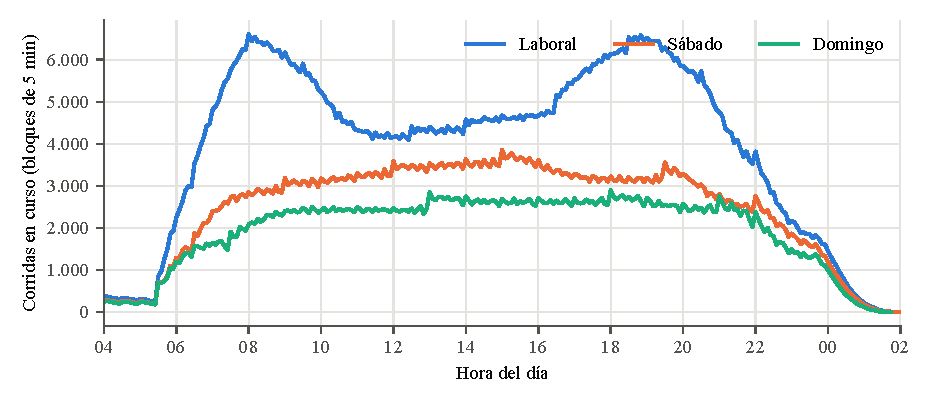
\includegraphics[width=\textwidth]{figures/corridas_dia.pdf}
\caption{Corridas en curso a lo largo del día, por tipo de día (bloques de 5 minutos).}
\label{fig:corridas-dia}
\end{figure}

Esta curva también sirvió para contrastar dos números del enunciado. La flota declarada de \FlotaDeclarada{} buses cubre apenas el \PctFlotaDeclarada\,\% de la punta laboral, de modo que no puede tomarse como límite, y el tamaño de la flota queda como decisión del modelo, tal como aclaró el equipo docente. Las \PlazasTotales{} plazas de los electroterminales también quedan muy por debajo de la flota necesaria.

\section{Energía, distancias e infraestructura}
\label{sec:energia-datos}

El consumo no viene en los datos. Se derivó de la batería y la autonomía nominal del bus, \Bateria~kWh entre \AutonomiaNominal~km, es decir \Consumo~kWh/km, igual con y sin pasajeros. Con la reserva de \PctReserva\,\%, la autonomía útil es de \Autonomia~km. A ese consumo, las corridas de un día laboral gastan \EnergiaServicioMwhLaboral~MWh.

Tampoco vienen los traslados en vacío. Se calcularon distancias viales dirigidas (sin suponer simetría ni línea recta) entre el final de cada corrida y el inicio de las demás, y entre esos puntos y los terminales y electroterminales. El tiempo de un traslado es su distancia a \VelocidadVacio~km/h, porque el enunciado no trae velocidades; las corridas mantienen su duración nominal.

Los cinco electroterminales son E1 Vespucio Norte (\PlazasUno{} plazas), E2 El Conquistador (\PlazasDos), E3 Los Espinos (\PlazasTres), E4 La Reina (\PlazasCuatro) y E5 Santa Rosa (\PlazasCinco), cada plaza con su conexión de \Potencia~kW. Para esperar y estacionar se usan cuatro terminales comunes existentes (T01 a T04), sin cargadores. La tarifa eléctrica es de USD~\TarifaMin{} por kWh de noche y sube hasta USD~\TarifaMax{} en los tramos de 14 a 17 y de 19 a 22~h.

Cada ruta se asigna al electroterminal con la menor suma de distancias por calle entre él y las cabeceras de la ruta (la salida hacia el inicio y la vuelta desde el final). Así quedan cinco sectores de \RutasSectorUno, \RutasSectorDos, \RutasSectorTres, \RutasSectorCuatro{} y \RutasSectorCinco{} rutas (Figura~\ref{fig:sectores}). El sector ordena el problema, pero los electroterminales siguen siendo compartidos por todos los buses.

\begin{figure}[htbp]
\centering
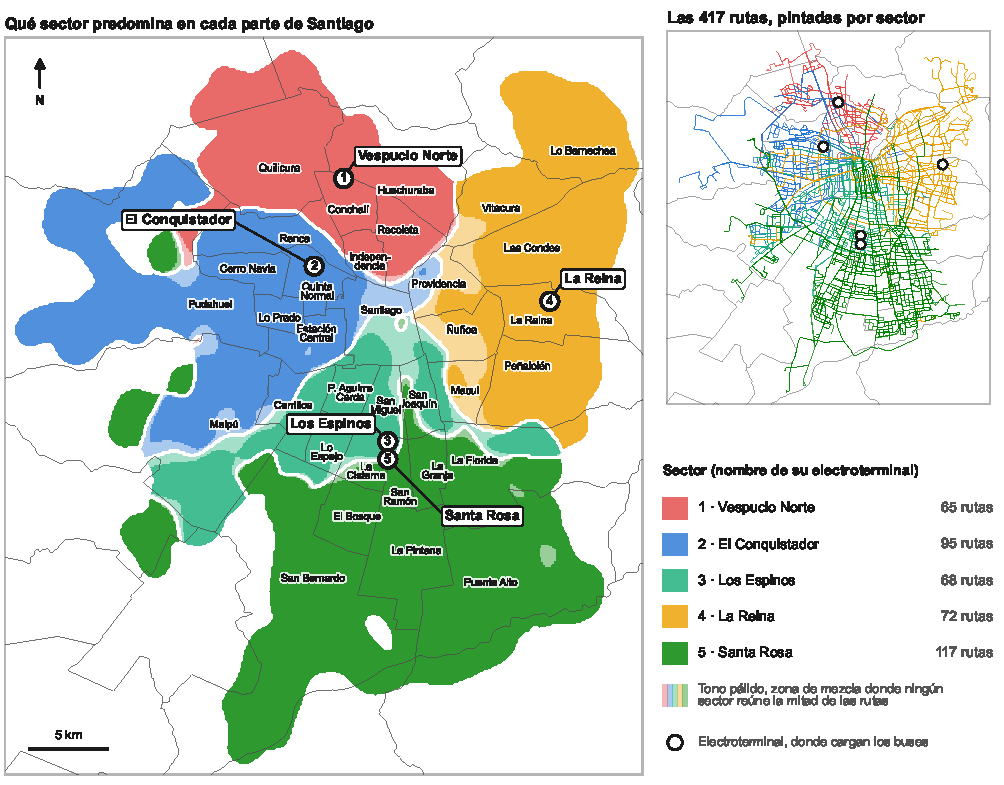
\includegraphics[width=.82\textwidth]{figures/mapa_sectores.pdf}
\caption{Sectores. Cada ruta queda asociada al electroterminal más cercano a sus cabeceras, medido por calle.}
\label{fig:sectores}
\end{figure}

\section{Datos que faltan, sesgos y cómo condicionan el modelo}
\label{sec:sesgos}

El diccionario de datos documenta \CamposDocumentados{} campos, pero \CamposAusentes{} de ellos no aparecen en ningún archivo, entre otros la potencia de los transformadores (\texttt{transformer\_mw}), los tiempos y distancias de traslado y el número de cargadores. La Tabla~\ref{tab:preparacion} resume las decisiones de preparación y cómo condicionan el modelo y los resultados.

\begin{table}[htbp]
\centering
\caption{Decisiones de preparación de los datos, riesgo de sesgo y efecto en el modelo.}
\label{tab:preparacion}
\small
\begin{tabularx}{\textwidth}{@{}p{3.6cm} X@{}}
\toprule
Decisión & Riesgo y efecto en el modelo \\
\midrule
Expandir las frecuencias (ec.~\ref{eq:salidas}) & Las salidas son representativas y no horarios observados. Fijan los huecos donde un bus puede encadenar o cargar. \\
Duraciones nominales, sin tráfico & Una conexión es factible o no, sin holgura. Con congestión, conexiones justas dejarían de serlo. Se evalúa con simulación (sección~\ref{sec:incertidumbre}). \\
Consumo lineal de \Consumo~kWh/km & Ignora pendiente, clima, pasajeros y degradación, y un error cambia directamente la flota. Se sensibiliza (sección~\ref{sec:sens-bus}). \\
Traslados a \VelocidadVacio~km/h & Define qué conexiones llegan a tiempo y cuánto cuesta reposicionar. Igual para el caso base y el método. \\
Límite eléctrico = conexiones $\times$ \Potencia~kW & El transformador no viene en los datos. Durante el día casi no se carga, así que afecta sobre todo la noche (sección~\ref{sec:repetibilidad}). \\
Terminales comunes sin límite de plazas & El enunciado no da su capacidad, y con un límite algunos buses terminarían más lejos (sección~\ref{sec:supuestos}). \\
Día aislado con batería llena & Lo fija el enunciado para ambos planes y favorece planes que terminan con poca energía (sección~\ref{sec:repetibilidad}). \\
Sectores fijos & Reduce el tamaño de cada búsqueda y evita cruzar la ciudad, pero impide combinar corridas de sectores vecinos. \\
\bottomrule
\end{tabularx}
\end{table}

Ninguna de estas decisiones favorece al método frente al caso base, porque ambos usan las mismas corridas, distancias, velocidad, terminales y batería inicial. Sí condicionan la lectura de los resultados, porque los planes son factibles dentro del modelo y no necesariamente en la operación real (capítulos~\ref{ch:sensibilidad} y~\ref{ch:piloto}).


\chapter[REVISIÓN BIBLIOGRÁFICA Y EVOLUCIÓN METODOLÓGICA]{Revisión bibliográfica y evolución metodológica} \label{ch:literatura}
% Capítulo 4. Revisión bibliográfica y evolución metodológica (rúbrica: revisión 5 pts y parte de estrategia 15 pts).

\section{Revisión crítica de las familias de métodos}
\label{sec:familias}

El problema del capítulo~\ref{ch:problema} pertenece a la familia de programación de vehículos eléctricos (E-VSP). \citeA{perumal_evspreview_2022} ordenan esa literatura según qué decisiones se toman en conjunto, entre ellas asignar corridas a buses, programar la carga, ubicar cargadores y dimensionar la flota. Este caso exige las dos primeras a la vez, con varios depósitos, carga parcial y cargadores finitos, sobre una red de decenas de miles de corridas. Con ese criterio se evaluó cada familia de métodos (Tabla~\ref{tab:familias}).

\begin{table}[htbp]
\centering
\caption{Familias de métodos revisadas, contrastadas con el caso.}
\label{tab:familias}
\footnotesize
\begin{tabularx}{\textwidth}{@{}p{2.3cm} X X p{2.4cm}@{}}
\toprule
Familia & Fortaleza & Debilidad o supuesto que choca con el caso & Referencias \\
\midrule
Flujo en red tiempo-espacio & Exacta y la que mejor escala sin batería; agrega arcos de espera y reduce el modelo. & Con la batería deja de ser un flujo puro; la energía se agrega después o como dimensión del nodo. & \citeA{kliewer_timespacemdvsp_2006}; \citeA{olsen_flowdecomposition_2022} \\
Generación de columnas y \emph{branch-and-price} & Óptimo con cota; trata carga parcial y cargadores finitos. & El mayor caso publicado resuelto al óptimo tiene 101 corridas; la red tiene tres órdenes de magnitud más. & \citeA{devos_capacitatedcharging_2024}; \citeA{wu_waitingtimebranchprice_2025}; \citeA{li_limitedenergy_2014} \\
Metaheurísticas y búsqueda en vecindarios grandes & Escalan a redes reales y entregan planes factibles desde temprano. & No traen cota propia, así que no indican qué tan lejos quedan del óptimo. & \citeA{wen_alnsevsp_2016}; \citeA{limmer_lnsevfleet_2023}; \citeA{ahuja_vlsn_2002} \\
Descomposición de Benders & Separa inversión (flota, cargadores) de operación. & Aquí la flota y la infraestructura vienen dadas y no hay un nivel de inversión que separar. & \citeA{legault_bendersfleetelectrification_2025} \\
Modelos con incertidumbre & Consumo y tiempos aleatorios dentro del modelo. & Los datos no traen distribuciones y el cómputo se multiplica. & \citeA{ricard_chanceconstrained_2026} \\
Simulación & Mide qué tan frágil es un plan. & No optimiza; solo evalúa. & --- \\
\bottomrule
\end{tabularx}
\end{table}

Los métodos exactos garantizan el óptimo, pero no llegan al tamaño de la red. \citeA{wu_waitingtimebranchprice_2025} resuelven al óptimo instancias de hasta 101 corridas y \citeA{devos_capacitatedcharging_2024}, que tratan la variante con cargadores finitos y carga parcial, siguen lejos de las \CorridasLaboral{} corridas del día laboral. Las metaheurísticas sí escalan, y \citeA{wen_alnsevsp_2016} muestran que una búsqueda adaptativa en vecindarios grandes resuelve el E-VSP con varios depósitos y carga parcial. Sin embargo, ninguna de las fuentes revisadas de esa familia modela cargadores finitos ni entrega una cota. Benders no aplica porque no se decide inversión, y para el modelo con incertidumbre faltan distribuciones, así que la robustez, que sigue siendo un tema abierto en el área \cite{wang_bevretrospective_2025}, se estudia con sensibilidad y simulación.

\section{Programar primero y cargar después}
\label{sec:evolucion}

Una estrategia común en la literatura es secuencial. Primero se arman cadenas de corridas como si los buses fueran diésel y después se les agrega la carga \cite{perumal_evspreview_2022}. \citeA{olsen_flowdecomposition_2022} la aplican en redes grandes. Resuelven un flujo en red tiempo-espacio sin batería, lo descomponen en cadenas con reglas que anticipan la energía y recién al final insertan las cargas, agregando buses donde la energía no alcanza. Su ventaja es la escala, y su riesgo es que el flujo no ve la batería, de modo que la fase de carga debe cortar cadenas y agregar buses. \citeA{perumal_evspreview_2022} distinguen los enfoques secuenciales de los integrados, que deciden corridas y carga a la vez y capturan su interacción a cambio de modelos más difíciles, y \citeA{vankootenniekerk_schedulingev_2017} formulan ese problema integrado con carga parcial.

Este proyecto midió ese riesgo en su propio caso. El prototipo de la Entrega~1 siguió la estrategia secuencial de \citeA{olsen_flowdecomposition_2022} sobre la muestra de \EdosRutasMuestra{} rutas. El flujo sin batería, que es una relajación del problema, encadenó las corridas con \EdosFlotaFaseUno{} buses. Cuando se exigió que cada bus tuviera energía para sus corridas, como obliga el problema, la flota subió a \EdosBusesPrototipoSinMejora{} (\EdosAumentoBateria{} buses más, +\EdosPctAumentoBateria\,\%). Ese aumento se explica por haber ignorado la batería al encadenar las corridas. Una construcción que revisa horario y energía en cada asignación logró \EdosBusesConstruccion{} buses factibles con las mismas corridas, de modo que al menos \EdosEvitables{} de los buses agregados se podían evitar reorganizando las jornadas (Tabla~\ref{tab:evolucion}). De ahí sale la decisión central del método, que es considerar la energía al armar cada jornada y no después.

\section{Evolución del método entre las entregas}
\label{sec:evolucion-entregas}

La Tabla~\ref{tab:evolucion} sigue el método a lo largo del semestre. En la Entrega~1 se eligió la red tiempo-espacio por sectores. En la Entrega~2 el diagnóstico anterior llevó a la construcción cronológica con energía y a una mejora local por pares y tríos de jornadas, con un modelo entero que decide las recargas. En la muestra de \EdosRutasMuestra{} rutas logró \EdosBusesModelo{} buses contra \EdosBusesBase{} del caso base (\EdosDeltaPctBuses\,\%). En la Entrega~3 el método se llevó a la red completa y los tres tipos de día, se generalizó la mejora a grupos de 3 a 8 buses elegidos parecidos o al azar, y se agregó un modelo exacto para medir la distancia al óptimo.

\begin{table}[htbp]
\centering
\caption{Evolución del método sobre la misma muestra de \EdosRutasMuestra{} rutas y \EdosCorridasMuestra{} corridas laborales (Entregas 1 y 2) y en la red completa (Entrega 3).}
\label{tab:evolucion}
\small
\begin{tabularx}{\textwidth}{@{}l X r@{}}
\toprule
Entrega & Método & Buses \\
\midrule
1 & Flujo en red tiempo-espacio sin batería (relajación, no operable) & \EdosFlotaFaseUno \\
1 & + descomposición en cadenas y carga insertada después & \EdosBusesPrototipoSinMejora \\
1--2 & + reparaciones y mejora por pares y tríos (prototipo final) & \EdosBusesPrototipo \\
2 & Construcción cronológica con energía, sin mejora & \EdosBusesConstruccion \\
2 & + mejora por pares y tríos con MILP de recargas & \EdosBusesModelo \\
\midrule
3 & Red completa, plan inicial (construcción cronológica) & \BusesInicialLaboral \\
3 & + pares y tríos, 40 min & \BusesMetodoParesTrios \\
3 & + cuartetos al azar, 40 min (método final) & \BusesPlanLaboral \\
\bottomrule
\end{tabularx}
\fuente{Cifras de las Entregas 1 y 2 en \texttt{08-entrega2/informe2/cifras.tex} y de la Entrega 3 en \texttt{09-entrega3/octetos/resultados/red\_completa\_417\_L.csv}.}
\end{table}

\section{Justificación del método elegido}
\label{sec:justificacion}

El método final es una búsqueda en vecindarios grandes con reparación exacta que combina tres ideas con respaldo en la literatura.

La primera es construir con la energía a la vista. El plan inicial recorre las corridas en orden de salida y asigna cada una a un bus que llega a tiempo y tiene energía, como la heurística constructiva con que parte la búsqueda de \citeA{wen_alnsevsp_2016}.

La segunda es mejorar el plan con vecindarios grandes. Una búsqueda local mejora un plan cambiando una parte de él, y \citeA{ahuja_vlsn_2002} describen el dilema de fondo. Un vecindario más grande encuentra mejores cambios en cada intento, pero cada intento cuesta más, y solo conviene si se puede revisar rápido. En el E-VSP, \citeA{wen_alnsevsp_2016} destruyen y reconstruyen partes del plan, y \citeA{limmer_lnsevfleet_2023} reparan la parte destruida con un modelo entero, que es exactamente lo que hace aquí el MILP de recargas.

La tercera es medir el método contra el exacto. Como la búsqueda no trae cota, su calidad se mide resolviendo al óptimo casos chicos con el mismo costo y las mismas reglas, como se propuso desde el informe~1.


\chapter[MODELO DEL CASO Y SUPUESTOS]{Modelo del caso y supuestos} \label{ch:modelo}
% Capítulo 5. Modelo del caso y supuestos (rúbrica modelo 10 pts y supuestos 5 pts).

Este capítulo formaliza el problema como un programa lineal entero mixto (MILP) basado en conexiones entre corridas. Es el modelo que se resuelve de forma exacta en los casos chicos (sección~\ref{sec:calidad}) y, restringido a pocas jornadas, el que usa el método híbrido para decidir las recargas (capítulo~\ref{ch:estrategia}). La implementación está en \texttt{metodo\_hibrido/exacto.py}.

\section{Conjuntos y parámetros}
\label{sec:conjuntos}

Sea \(N\) el conjunto de corridas de un tipo de día. Cada corrida \(i\in N\) tiene una hora de inicio \(s_i\) y de término \(f_i\), un origen y un destino, una distancia de servicio \(L_i\) y un sector \(\sigma(i)\). Sean \(T\) los terminales comunes, \(E\) los electroterminales y \(F=T\cup E\) los lugares donde un bus puede terminar el día. Las distancias son viales y dirigidas, y el tiempo de un traslado en vacío es su distancia a la velocidad \(v\) de \VelocidadVacio~km/h.

Un bus que atiende la corrida \(i\) y después la \(j\) puede hacerlo de dos maneras. Si va directo, el par pertenece a
\[
A=\{(i,j)\in N\times N \mid \sigma(i)=\sigma(j),\ f_i+\tau_{ij}\le s_j\},
\]
donde \(\tau_{ij}\) es el tiempo del traslado entre el destino de \(i\) y el origen de \(j\), que mide \(d_{ij}\) kilómetros. Si en ese hueco pasa a cargar, elige una opción \(k\) de un catálogo \(K_{ij}\). Cada opción fija un electroterminal \(e(k)\), una ventana de carga dentro del hueco, los kilómetros de ida \(a_k\) y de vuelta \(h_k\), la energía máxima \(g_k\) que alcanza a cargar a \Potencia~kW en bloques completos de \MinutosBloque~minutos y el precio medio \(p_k\) de la energía en esa ventana. Una opción entra al catálogo solo si el bus alcanza a llegar, cargar al menos un bloque y llegar a tiempo al origen de \(j\). Se escribe \(R=\{(i,j,k)\mid k\in K_{ij}\}\).

Para cada corrida se conoce la distancia \(d^{0}_i\) desde el terminal común más cercano a su origen y, para cada lugar \(\ell\in F\) alcanzable dentro del horizonte, la distancia \(d^{1}_{i\ell}\) desde su destino. Los parámetros físicos son la capacidad de la batería \(B=\Bateria\)~kWh, la reserva \(m=\Reserva\)~kWh y el consumo \(r=\Consumo\)~kWh/km, igual con y sin pasajeros. Los económicos son \(c^{B}=\CostoBus\) USD por bus, \(c^{D}=\CostoKmUnit\) USD/km y \(c^{S}=\CostoSesion\) USD por sesión. Cada electroterminal \(e\) tiene \(P_e\) plazas y \(C_e\) conexiones. El día se divide en bloques \(\omega\in\Omega\) de \MinutosBloque~minutos, y \(\alpha_{k\omega}\) vale uno si la opción \(k\) está cargando durante el bloque \(\omega\).

\section{Variables de decisión}
\label{sec:variables}

El modelo usa seis familias de variables. La variable binaria \(u_i\) vale uno si la corrida \(i\) es la primera de una jornada, es decir, si con ella sale un bus nuevo, y \(z_{i\ell}\) vale uno si \(i\) es la última de una jornada y el bus termina en \(\ell\in F\). La binaria \(x_{ij}\) indica que un mismo bus hace \(i\) y luego \(j\) con un traslado directo, y \(y_{ijk}\) que lo hace pasando a cargar con la opción \(k\). La variable continua \(q_{ijk}\ge 0\) son los kWh que carga en esa opción, y \(e_i\in[m,B]\) es la energía que le queda al bus al terminar la corrida \(i\).

\section{Función objetivo}
\label{sec:objetivo}

El costo total del plan es
\begin{multline}
\min\ c^{B}\sum_{i\in N}u_i
+ c^{D}\Bigl(\sum_{i\in N}d^{0}_i u_i+\sum_{i\in N}\sum_{\ell\in F}d^{1}_{i\ell}z_{i\ell}
+\sum_{(i,j)\in A}d_{ij}x_{ij}+\sum_{(i,j,k)\in R}(a_k+h_k)\,y_{ijk}+\sum_{i\in N}L_i\Bigr)\\
+\sum_{(i,j,k)\in R}\bigl(c^{S}y_{ijk}+p_k\,q_{ijk}\bigr).
\label{eq:objetivo}
\end{multline}
El primer término cuenta los buses, porque cada jornada empieza en exactamente una corrida. El segundo suma todos los kilómetros, que son la salida desde el terminal, el regreso al final del día, los traslados entre corridas, los desvíos para cargar y los kilómetros de servicio, que son constantes. El último término es el costo de las sesiones y de la energía.

\section{Restricciones}
\label{sec:restricciones}

Cada corrida tiene exactamente un antecesor o es la primera de su jornada, y exactamente un sucesor o es la última,
\begin{align}
u_j+\sum_{(i,j)\in A}x_{ij}+\sum_{(i,j,k)\in R}y_{ijk} &= 1 && \forall j\in N, \label{eq:entra}\\
\sum_{\ell\in F}z_{j\ell}+\sum_{(j,l)\in A}x_{jl}+\sum_{(j,l,k)\in R}y_{jlk} &= 1 && \forall j\in N. \label{eq:sale}
\end{align}
Juntas, (\ref{eq:entra}) y (\ref{eq:sale}) dividen las corridas en cadenas disjuntas que empiezan y terminan una vez, que son las jornadas, y garantizan que cada corrida se cubra exactamente una vez. Como \(A\) y \(R\) solo unen corridas del mismo sector, ninguna jornada cruza sectores.

La energía se sigue a lo largo de cada cadena. Un bus parte lleno, y desde ahí cada conexión descuenta el traslado y la corrida siguiente,
\begin{align}
u_i=1 &\ \Rightarrow\ e_i\le B-r\,(d^{0}_i+L_i) && \forall i\in N, \label{eq:inicio}\\
x_{ij}=1 &\ \Rightarrow\ e_j\le e_i-r\,(d_{ij}+L_j) && \forall (i,j)\in A. \label{eq:directo}
\end{align}
Cuando el bus pasa a cargar, debe llegar al electroterminal sobre la reserva, no puede cargar más de lo que cabe en la batería ni más de lo que permite la ventana, y la energía de la corrida siguiente descuenta el desvío,
\begin{align}
y_{ijk}=1 &\ \Rightarrow\ e_i-r\,a_k\ge m,\qquad e_i-r\,a_k+q_{ijk}\le B && \forall (i,j,k)\in R, \label{eq:carga-llegada}\\
y_{ijk}=1 &\ \Rightarrow\ e_j\le e_i+q_{ijk}-r\,(a_k+h_k+L_j) && \forall (i,j,k)\in R, \label{eq:carga-balance}\\
q_{ijk} &\le g_k\,y_{ijk} && \forall (i,j,k)\in R. \label{eq:carga-max}
\end{align}
Al terminar el día, el bus debe llegar a su lugar final con la reserva intacta,
\begin{equation}
z_{i\ell}=1\ \Rightarrow\ e_i-r\,d^{1}_{i\ell}\ge m\qquad \forall i\in N,\ \ell\in F. \label{eq:final}
\end{equation}
Las implicancias (\ref{eq:inicio})--(\ref{eq:final}) se implementan como restricciones indicadoras de Gurobi y son equivalentes a restricciones lineales con constantes grandes. Que \(e_i\) se acote solo por arriba no es un problema, ya que el dominio \(e_i\ge m\) obliga a que la energía real nunca baje de la reserva.

Por último, en cada electroterminal y bloque no puede haber más buses cargando que conexiones, ni más buses presentes que plazas, contando los que cargan y los que ya terminaron su día ahí,
\begin{align}
\sum_{(i,j,k)\in R,\ e(k)=e}\alpha_{k\omega}\,y_{ijk} &\le C_e && \forall e\in E,\ \omega\in\Omega, \label{eq:conexiones}\\
\sum_{(i,j,k)\in R,\ e(k)=e}\alpha_{k\omega}\,y_{ijk}+\sum_{i\in N,\ f_i+\tau_{ie}\le \omega}z_{ie} &\le P_e && \forall e\in E,\ \omega\in\Omega. \label{eq:plazas}
\end{align}
Los dominios son \(u,z,x,y\in\{0,1\}\), \(q\ge 0\) y \(m\le e\le B\).

\section{Tamaño del modelo y modelo podado}
\label{sec:tamano}

El modelo es exacto pero no escala. Solo dentro de cada sector hay unos \ParesSectorMillones{} millones de pares de corridas en un día laboral, y cada par que deja un hueco suficiente abre además varias opciones de carga. En los casos de prueba, la versión completa con \CorridasRutasMediano{} corridas ya necesitó unos 13~GB de memoria, más de lo que tiene el equipo usado. Para llegar a casos medianos se usó una versión podada, que deja en cada par solo las opciones de carga no dominadas (las que no tienen otra con menos kilómetros, más energía posible y un precio igual o menor) y omite (\ref{eq:conexiones}) y (\ref{eq:plazas}). Cualquier plan que use una opción dominada se puede cambiar por la que la domina cargando lo mismo, así que la poda no cambia el óptimo del modelo sin capacidades. Si el plan óptimo del modelo podado pasa después el auditor, que sí revisa plazas y conexiones, ese plan es óptimo también para el modelo completo. Así ocurrió en todos los casos medianos reportados en la sección~\ref{sec:calidad}.

\section{Supuestos}
\label{sec:supuestos}

La Tabla~\ref{tab:supuestos} reúne los supuestos del modelo que no vienen fijados por los datos o el enunciado, con su justificación, cómo afectan la comparación y dónde se pone a prueba cada uno. Ninguno favorece al método frente al caso base, porque ambos se construyen sobre las mismas corridas, distancias, velocidad, terminales y batería inicial.

\begin{table}[htbp]
\centering
\caption{Supuestos del modelo, su justificación y cómo se evaluaron.}
\label{tab:supuestos}
\footnotesize
\begin{tabularx}{\textwidth}{@{}p{3cm} X X p{2.1cm}@{}}
\toprule
Supuesto & Justificación & Efecto si no se cumple & Dónde se evalúa \\
\midrule
Tiempos de viaje del GTFS, sin tráfico ni mantenciones & Los datos no traen variabilidad ni fallas & Las conexiones justas se rompen y el plan se atrasa más que el caso base & Simulación, sección~\ref{sec:incertidumbre} \\
Consumo lineal de \Consumo~kWh/km & Se deriva de la batería y la autonomía nominal & Más consumo exige más buses en ambos planes & Sensibilidad, sección~\ref{sec:sens-bus} \\
Batería de \Bateria~kWh y reserva de \PctReserva\,\% & Valores del enunciado & Baterías más chicas obligan a recargar más & Sensibilidad y recarga forzada \\
Carga lineal hasta \Potencia~kW, en bloques de \MinutosBloque~min & No hay curva de carga en los datos & La carga real se frena cerca del 100\,\%; el plan carga poco y lejos de ese tramo & Discusión, sección~\ref{sec:limitaciones} \\
Límite eléctrico igual a conexiones por \Potencia~kW & \texttt{transformer\_mw} no viene en ningún archivo & De día casi no se carga; afecta sobre todo la noche & Mitad de conexiones y repetibilidad \\
Traslados en vacío a \VelocidadVacio~km/h & El enunciado no trae velocidades & Más rápido acortaría traslados y bajaría buses en ambos planes & No se varió (limitación) \\
Terminales comunes sin límite de plazas & El enunciado no da su capacidad & Con un límite, algunos buses terminarían más lejos y sumarían km & Ocupación medida, abajo \\
Día aislado con batería llena & Lo fija el enunciado, igual para ambos planes & El día no se repite solo & Repetibilidad, sección~\ref{sec:repetibilidad} \\
Espera sin costo & Pesa igual en ambos planes y achica el modelo & Suma cerca del \PctEspera\,\% al costo & Sensibilidad de precios \\
Sectores fijos & Achican cada búsqueda y evitan cruzar la ciudad & Se pierden combinaciones entre sectores vecinos & Extensión, sección~\ref{sec:extensiones} \\
\bottomrule
\end{tabularx}
\end{table}

La corrección del informe~2 preguntó qué pasa si los terminales comunes tienen una capacidad realista. Para responderla se midió cuántos buses llegan a estar a la vez en cada uno (\texttt{09-entrega3/kpi/ocupacion\_terminales.py}). En el plan del día laboral, el máximo va de \TerminalMinPlan{} a \TerminalMaxPlan{} buses por terminal, siempre de noche, cuando la mayoría de la flota está estacionada, y en el caso base va de \TerminalMinBase{} a \TerminalMaxBase. Son cifras muy por encima de lo que cabe en un terminal real, de modo que el supuesto no favorece al método, pero sí esconde un problema que ambos planes comparten, que es dónde guardar de noche una flota de varios miles de buses. En la práctica eso se resuelve repartiendo los buses entre los depósitos de los operadores, y si cada terminal tuviera un tope, los buses que no caben tendrían que terminar en otro lugar más lejano, con más kilómetros en vacío en ambos planes. Es una extensión directa del modelo, porque bastaría agregar a (\ref{eq:plazas}) una restricción análoga para cada terminal común.


\chapter[ESTRATEGIA DE SOLUCIÓN E IMPLEMENTACIÓN]{Estrategia de solución e implementación} \label{ch:estrategia}
% Capítulo 6. Estrategia de solución e implementación (rúbrica estrategia 15 pts e implementación 5 pts).

Como el modelo del capítulo~\ref{ch:modelo} no se puede resolver para la red completa, el plan se obtiene con un método híbrido que arma una solución factible y luego la mejora por partes. La Figura~\ref{fig:flujo} muestra el procedimiento completo, sin detalles de código, y las secciones siguientes explican cada paso.

\begin{figure}[htbp]
\centering
\begin{tikzpicture}[node distance=14mm and 5mm,
  caja/.style={draw, rounded corners, align=center, font=\footnotesize, minimum height=11mm, text width=25mm},
  dato/.style={caja, fill=black!5}, flecha/.style={-Stealth}]
\node[dato] (dat) {Corridas, distancias\\ y parámetros};
\node[caja, right=of dat] (sec) {Sectores\\{\scriptsize cada ruta a su\\ electroterminal}};
\node[caja, right=of sec] (ini) {Plan inicial\\{\scriptsize corridas en orden\\ de salida}};
\node[caja, right=of ini] (sor) {Sorteo de\\ cuatro buses\\{\scriptsize del mismo sector}};
\node[caja, below=of sor] (mov) {Propuestas\\{\scriptsize absorción\\ y rotación}};
\node[caja, left=of mov] (milp) {MILP local\\{\scriptsize terminales y recargas\\ de las cuatro\\ jornadas}};
\node[caja, left=of milp] (aud) {Auditor\\{\scriptsize se acepta si es\\ factible y más barato}};
\node[dato, left=of aud] (sal) {Plan final\\{\scriptsize jornada de cada bus\\ e indicadores}};
\draw[flecha] (dat) -- (sec);
\draw[flecha] (sec) -- (ini);
\draw[flecha] (ini) -- (sor);
\draw[flecha] (sor) -- (mov);
\draw[flecha] (mov) -- (milp);
\draw[flecha] (milp) -- (aud);
\draw[flecha, dashed] (aud.north) to[out=80, in=200] node[pos=.55, fill=white, font=\scriptsize, inner sep=1pt]{se repite hasta agotar el tiempo} (sor.south west);
\draw[flecha] (aud) -- (sal);
\end{tikzpicture}
\caption{Procedimiento del método híbrido. La búsqueda repite el sorteo, las propuestas, el MILP local y la auditoría hasta agotar su tiempo, y el plan que sale siempre es factible.}
\label{fig:flujo}
\end{figure}

\section{Sectores y plan inicial}
\label{sec:construccion}

El primer paso asocia cada ruta a un electroterminal, como se describió en la sección~\ref{sec:energia-datos}. Cada bus atiende corridas de un solo sector, aunque puede cargar en cualquier electroterminal.

El plan inicial se arma recorriendo las corridas en orden de hora de salida. Para cada una se revisan los buses del sector que ya están en servicio y se descartan los que no alcanzan a llegar a tiempo a su origen o no tienen energía suficiente para el traslado, la corrida y un regreso de respaldo a un terminal sin bajar de la reserva. Entre los que quedan se elige el de menor traslado en vacío. Si a un bus le falta energía, se intenta intercalar una visita a un electroterminal en el hueco previo, cargando solo lo necesario y verificando que haya plaza y conexión durante toda la visita. Si ningún bus puede tomar la corrida, se agrega uno nuevo, con la batería llena, desde el terminal común más cercano. Este paso no usa optimización y toma \SegundosInicial~segundos para el día laboral completo.

Frente al caso base, el plan inicial ya cambia tres cosas. Comparte buses entre todas las rutas del sector, carga solo la energía que falta en vez de llenar la batería, y elige el bus que queda más cerca. Con eso logra \BusesInicialLaboral{} buses en día laboral, y explica el \PctAhorroInicial\,\% de la reducción total de flota (sección~\ref{sec:origen-ahorro}).

\section{Mejora por grupos de buses}
\label{sec:mejora}

La mejora toma grupos de cuatro jornadas del mismo sector y busca una forma más barata de repartir sus corridas. Los cuatro buses se sortean con una semilla fija, lo que permite repetir exactamente una corrida del método. Dentro del grupo se prueban dos operaciones, que muestra la Figura~\ref{fig:operaciones}.

\begin{figure}[htbp]
\centering
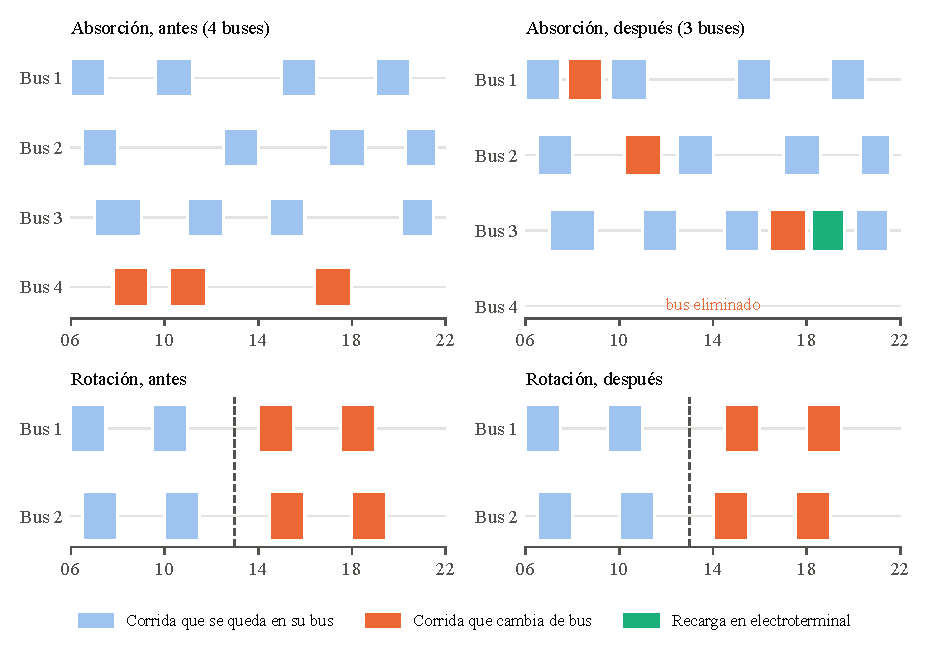
\includegraphics[width=\textwidth]{figures/operaciones.pdf}
\caption{Las dos operaciones de la mejora, con horarios ilustrativos. En la absorción, el bus con menos corridas las reparte entre los otros tres y, si al bus 3 ya no le alcanza la batería, el MILP local le agrega una recarga. En la rotación, dos buses intercambian todo lo que hacen después de un corte (línea punteada).}
\label{fig:operaciones}
\end{figure}

En la absorción, el bus que menos corridas tiene intenta repartirlas entre los otros tres. Cada corrida se inserta en un hueco compatible de algún receptor, y como hay muchas formas de hacerlo se conservan solo unas pocas alternativas parciales, ordenadas por kilómetros en vacío y por lo pareja que queda la carga de trabajo. Si todas las corridas encuentran lugar, el grupo pasa de cuatro buses a tres, y el plan ahorra USD~\CostoBus{} diarios más lo que cambien los kilómetros y la energía. En la rotación, cada jornada se corta en un punto y las partes finales se intercambian entre los buses, sin tocar los comienzos. La rotación no elimina buses, pero puede acortar traslados o dejar espacio para una absorción posterior.

\section{El MILP local y la aceptación}
\label{sec:milp-local}

Cada propuesta define qué corridas hace cada bus y en qué orden, pero todavía no dice si los buses tienen energía para hacerlas ni dónde cargan. Ese es el papel del MILP local. Con las corridas de cada jornada ya fijas, decide en qué terminal parte cada bus, si recarga en cada hueco, en qué electroterminal y cuánto, y dónde termina el día. Lo hace minimizando los kilómetros en vacío, las sesiones y el costo de la energía, y respetando el balance de energía, la reserva, la capacidad de la batería, la potencia de carga y la capacidad que dejan libre en cada electroterminal los buses que no están en el grupo. Es el modelo del capítulo~\ref{ch:modelo} con el orden de las corridas fijo y restringido a cuatro jornadas, y su formulación completa está en el anexo~\ref{an:milp-local}.

Se resuelve con Gurobi, con un límite de dos segundos por intento, una tolerancia de 2\,\% y un hilo. Si no encuentra solución factible, la propuesta se descarta. Si la encuentra, el plan candidato se reconstruye y el auditor lo revisa completo. El cambio se acepta solo si el auditor lo aprueba y el costo total baja. Por eso la búsqueda nunca empeora el plan y puede detenerse en cualquier momento con un plan factible. En la corrida final del día laboral, cada semilla probó en promedio \IntentosCuartetos{} propuestas en \MinutosFinal{} minutos y aceptó \MejorasCuartetos.

\section{Por qué cuatro buses elegidos al azar}
\label{sec:por-que-cuartetos}

El tamaño del grupo es el dilema que describen \citeA{ahuja_vlsn_2002}. Un grupo más grande ofrece más formas de repartir las corridas, pero cada propuesta tarda más en resolverse y en el mismo tiempo se prueban menos. Para elegirlo se compararon grupos de 2 a 8 buses, elegidos al azar o por tener horarios parecidos, todos con el mismo tiempo y en el mismo computador, en la red completa y en casos chicos con óptimo conocido. La regla acordada por el grupo fue quedarse con el método más barato a igual tiempo. Ganó el grupo de cuatro buses elegidos al azar, y los detalles están en la sección~\ref{sec:metodo-elegido}.

\section{Validación con el modelo exacto}
\label{sec:validacion}

Para medir la calidad del método se resolvió el modelo del capítulo~\ref{ch:modelo} al óptimo en casos chicos, de 2 a 4 rutas de un mismo sector, y en casos medianos de 6 a 12 rutas con la versión podada. Los casos usan las mismas corridas, distancias, costos y reglas que la red completa, así que el óptimo es una vara directa. Además, como con la batería de \Bateria~kWh casi ningún bus necesita recargar en esos casos, se crearon copias con baterías de 150 y 120~kWh para obligar a recargar y probar el método donde la carga sí pesa. Con 100~kWh ya no hay solución, porque algunas corridas, contando el traslado de salida y el de regreso, necesitan entre 105 y 112~kWh.

\section{Implementación y herramientas}
\label{sec:implementacion}

Todo está escrito en Python. Los modelos enteros se resuelven con Gurobi~12 a través de \texttt{gurobipy}, con licencia académica, porque la licencia gratuita que trae el paquete solo admite modelos de hasta dos mil variables y no alcanza para grupos de tres buses o más. El método está en la carpeta \texttt{metodo\_hibrido} del repositorio, el caso base en \texttt{codigo/tres\_fases} y los estudios de la Entrega~3 en \texttt{09-entrega3}. Todo se corrió en un mismo computador (Mac M1 con 8~GB de memoria), porque la búsqueda se corta por reloj y depende del equipo.

El auditor (\texttt{verificar.py}) es independiente del constructor y de la búsqueda. Reconstruye cada plan desde sus actividades y comprueba que cada corrida se cubra una vez con su horario, que cada bus llegue a tiempo a su siguiente actividad, que ninguna jornada cruce sectores, que la energía no baje de la reserva, que no se excedan plazas ni conexiones y que el costo informado coincida con el recalculado. Ningún plan de este informe se usó sin pasar por él, incluidos los del caso base y los del modelo exacto.

Cada corrida guarda sus parámetros, las versiones del software y una huella SHA-256 de cada archivo de entrada y de código. Un script genera todas las cifras del informe desde los resultados, y el anexo~\ref{an:reproduccion} indica cómo repetir cada una.


\chapter[CASO BASE]{Caso base} \label{ch:caso-base}
% Capítulo 7. Caso base (rúbrica 10 pts).

El caso base es la referencia contra la que se miden todos los indicadores. Representa una forma razonable de programar la flota sin investigación operativa, y por eso incluye la recarga, que es parte esencial del problema, como pidió el equipo docente en la Entrega~2.

\section{Política miope por ruta con recarga}
\label{sec:politica-miope}

La política decide corrida por corrida sin mirar las que vienen, y por eso se le llama miope. Las corridas se recorren en orden de hora de salida y cada ruta tiene sus propios buses, de modo que un bus nunca atiende dos rutas distintas aunque sean del mismo sector. Cada corrida se asigna al bus de su ruta que lleva más tiempo libre y alcanza a llegar a tiempo. Si la batería de ese bus no alcanza para la corrida y el regreso a un terminal con la reserva de \Reserva~kWh, el bus va antes al electroterminal más cercano con cupo y carga hasta el 100\,\% a la tarifa de esa hora. Si ningún bus de la ruta puede tomar la corrida, se agrega uno nuevo con la batería llena desde el terminal común más cercano, y al terminar su última corrida cada bus vuelve al terminal común más cercano. La implementación está en \texttt{codigo/tres\_fases/caso\_base.py}.

\section{Por qué es una referencia defendible}
\label{sec:caso-base-defendible}

La política reproduce cómo se programaría una flota eléctrica con la lógica de una flota diésel, con buses asignados a una ruta que cargan cuando se les acaba la energía. No resuelve ningún modelo, así que toda diferencia con el método viene de coordinar mejor las decisiones. Se compara en las mismas condiciones, con las mismas corridas, distancias, velocidad en vacío, costos, electroterminales y batería inicial, y lee la batería, la reserva y el consumo de los mismos parámetros que el método, lo que permite compararlos también en la sensibilidad. Su plan pasó por el mismo auditor que los planes del método, que confirmó la cobertura, la continuidad, la energía, las capacidades y el costo.

Para no inflar el ahorro se eligió la versión más favorable al caso base. La política admite un umbral, de modo que con un umbral de 30\,\% el bus va a cargar apenas su batería baja de ese nivel, aunque todavía le alcance para la corrida siguiente. En la muestra de \EdosRutasMuestra{} rutas, subir el umbral solo empeoró el caso base, porque multiplica las visitas a los electroterminales. Con umbrales de 0, 20, 30 y 50\,\% necesitó \EdosBusesBase, \EdosBusesUmbralVeinte, \EdosBusesUmbralTreinta{} y \EdosBusesUmbralCincuenta{} buses, de modo que se usa el umbral de 0\,\%.

Este caso base reemplazó al que se mostró en la presentación de la Entrega~2, que no recargaba, porque exageraba la ganancia de cualquier método que sí cargara.

\section{Resultado en la red completa}
\label{sec:resultado-caso-base}

La Tabla~\ref{tab:caso-base} resume el caso base en los tres tipos de día. En día laboral necesita \BusesBaseLaboral{} buses y cuesta USD~\CostoBaseLaboral{} al día.

\begin{table}[htbp]
\centering
\caption{Caso base en la red completa por tipo de día. Costos en USD por día y su porcentaje del costo total.}
\label{tab:caso-base}
\small
\begin{tabular}{@{}lrrrrrr@{}}
\toprule
 & \multicolumn{2}{c}{Laboral} & \multicolumn{2}{c}{Sábado} & \multicolumn{2}{c}{Domingo} \\
\cmidrule(lr){2-3}\cmidrule(lr){4-5}\cmidrule(lr){6-7}
Indicador & Valor & \% & Valor & \% & Valor & \% \\
\midrule
Buses & \BusesBaseLaboral & & \BusesBaseSabado & & \BusesBaseDomingo & \\
Costo total & \CostoBaseLaboral & 100 & \CostoBaseSabado & 100 & \CostoBaseDomingo & 100 \\
\quad Buses & \CostoFlotaBaseLaboral & \PctFlotaBaseLaboral & \CostoFlotaBaseSabado & \PctFlotaBaseSabado & \CostoFlotaBaseDomingo & \PctFlotaBaseDomingo \\
\quad Kilómetros & \CostoKmBaseLaboral & \PctKmBaseLaboral & \CostoKmBaseSabado & \PctKmBaseSabado & \CostoKmBaseDomingo & \PctKmBaseDomingo \\
\quad Energía & \CostoEnergiaBaseLaboral & \PctEnergiaBaseLaboral & \CostoEnergiaBaseSabado & \PctEnergiaBaseSabado & \CostoEnergiaBaseDomingo & \PctEnergiaBaseDomingo \\
\quad Sesiones & \CostoSesionesBaseLaboral & \PctSesionesBaseLaboral & \CostoSesionesBaseSabado & \PctSesionesBaseSabado & \CostoSesionesBaseDomingo & \PctSesionesBaseDomingo \\
Km en vacío (\% de los km) & \PctVacioBaseLaboral & & \PctVacioBaseSabado & & \PctVacioBaseDomingo & \\
Corridas por bus & \CorridasPorBusBaseLaboral & & \CorridasPorBusBaseSabado & & \CorridasPorBusBaseDomingo & \\
\bottomrule
\end{tabular}
\fuente{Planes en \texttt{codigo/output/tres\_fases/red\_417\_\{L,S,D\}\_caso\_base} e indicadores en \texttt{09-entrega3/kpi/resultados/kpi\_planes.csv}.}
\end{table}

La composición del costo dice dónde está el margen de mejora. Los buses son el \PctFlotaBaseLaboral\,\% del costo del día laboral, y como cada ruta tiene sus propios buses, muchos pasan buena parte del día esperando la siguiente salida de su ruta mientras otra ruta cercana necesita un bus. Ese es el componente más mejorable, y el que ataca primero el método al compartir buses entre las rutas de un sector. Los kilómetros son el \PctKmBaseLaboral\,\% y de ellos el \PctVacioBaseLaboral\,\% se recorre sin pasajeros, porque cada ruta reposiciona sus propios buses. La energía y las sesiones pesan poco en el costo, \PctEnergiaBaseLaboral{} y \PctSesionesBaseLaboral\,\%, pero no son irrelevantes, porque deciden cuándo un bus tiene que salir de servicio. El caso base carga siempre hasta el 100\,\% y lo hace sobre todo entre las 19 y las 22 horas, cuando la tarifa es más alta (sección~\ref{sec:uso-e}).


\chapter[RESULTADOS Y ANÁLISIS]{Resultados y análisis} \label{ch:resultados}
% Capítulo 8. Resultados y análisis (rúbrica 50 pts).

Este capítulo presenta el plan del método para los tres tipos de día, explica de dónde sale el ahorro, justifica la elección de cuartetos al azar y mide qué tan cerca del óptimo queda la solución. Salvo que se diga otra cosa, el plan es el de cuartetos al azar con \MinutosFinal{} minutos de búsqueda por tipo de día y las cifras son el promedio de \SemillasPlanLaboral{} semillas.

\section{Resultado principal}
\label{sec:resultado-principal}

La Tabla~\ref{tab:resultado} compara el plan con el caso base. En día laboral, el plan cubre las mismas \CorridasLaboral{} corridas con \BusesPlanLaboral{} buses, \AhorroBusesLaboral{} menos que el caso base (\DeltaPctBusesLaboral\,\%), y cuesta USD~\CostoPlanLaboral{} al día, USD~\AhorroCostoLaboral{} menos (\DeltaPctCostoLaboral\,\%). El sábado y el domingo la reducción de buses es incluso mayor, \BajaBusesSabado{} y \BajaBusesDomingo\,\%. Si la semana se cuenta como cinco días laborales más un sábado y un domingo, el costo semanal pasa de USD~\CostoSemanaBaseMillones{} a \CostoSemanaPlanMillones{} millones, \BajaSemana\,\% menos. La flota que RED tendría que tener es la del día laboral, porque los otros días se cubren con una parte de ella.

\begin{table}[htbp]
\centering
\caption{Caso base y plan de cuartetos al azar en la red completa (promedio de tres semillas).}
\label{tab:resultado}
\small
\begin{tabular}{@{}lrrrrrr@{}}
\toprule
 & & \multicolumn{2}{c}{Buses} & \multicolumn{2}{c}{Costo (USD/día)} & \\
\cmidrule(lr){3-4}\cmidrule(lr){5-6}
Día & Corridas & Caso base & Plan & Caso base & Plan & $\Delta$ costo \\
\midrule
Laboral & \CorridasLaboral & \BusesBaseLaboral & \BusesPlanLaboral & \CostoBaseLaboral & \CostoPlanLaboral & \DeltaPctCostoLaboral\,\% \\
Sábado & \CorridasSabado & \BusesBaseSabado & \BusesPlanSabado & \CostoBaseSabado & \CostoPlanSabado & \DeltaPctCostoSabado\,\% \\
Domingo & \CorridasDomingo & \BusesBaseDomingo & \BusesPlanDomingo & \CostoBaseDomingo & \CostoPlanDomingo & \DeltaPctCostoDomingo\,\% \\
\midrule
Semana & & & & \CostoSemanaBase & \CostoSemanaPlan & \DeltaPctSemana\,\% \\
\bottomrule
\end{tabular}
\fuente{Plan en \texttt{09-entrega3/octetos/resultados/red\_completa\_417\_\{L,S,D\}.csv} y caso base en \texttt{09-entrega3/kpi/resultados/kpi\_planes.csv}. La semana suma cinco días laborales, un sábado y un domingo.}
\end{table}

\section{De dónde sale el ahorro}
\label{sec:origen-ahorro}

La Tabla~\ref{tab:pasos} sigue el día laboral paso a paso. El plan inicial, que todavía no optimiza nada, ya baja la flota de \BusesBaseLaboral{} a \BusesInicialLaboral{} buses (\DeltaPctBusesInicialLaboral\,\%). Así, el \PctAhorroInicial\,\% de la reducción total viene de compartir buses entre las rutas de un sector, de cargar solo lo necesario y de elegir el bus que queda más cerca, y no de la búsqueda. La mejora por grupos agrega el resto. Con pares y tríos, el método de la Entrega~2, llega a \BusesMetodoParesTrios{} buses, y con cuartetos al azar a \BusesPlanLaboral, \MejoraInicialLaboral\,\% de costo sobre el plan inicial. En sábado y domingo la búsqueda aporta más, \MejoraInicialSabado{} y \MejoraInicialDomingo\,\%, porque esos días los buses cargan más y la búsqueda tiene más recargas que reorganizar.

\begin{table}[htbp]
\centering
\caption{Buses y costo del día laboral en cada etapa.}
\label{tab:pasos}
\small
\begin{tabular}{@{}lrrr@{}}
\toprule
Etapa & Buses & Costo (USD/día) & $\Delta$ costo contra el caso base \\
\midrule
Caso base miope & \BusesBaseLaboral & \CostoBaseLaboral & --- \\
Plan inicial del método & \BusesInicialLaboral & \CostoInicialLaboral & \DeltaPctCostoInicialLaboral\,\% \\
Mejora por pares y tríos, \MinutosFinal{} min & \BusesMetodoParesTrios & \CostoMetodoParesTrios & \\
Mejora por cuartetos al azar, \MinutosFinal{} min & \BusesPlanLaboral & \CostoPlanLaboral & \DeltaPctCostoLaboral\,\% \\
\bottomrule
\end{tabular}
\end{table}

Por componente, cerca de tres de cada cuatro dólares ahorrados son buses (Figura~\ref{fig:ahorro}). Los buses aportan USD~\AhorroCompFlota{} diarios, el \PctAhorroCompFlota\,\% del ahorro, la energía USD~\AhorroCompEnergia{} y los kilómetros USD~\AhorroCompKm. Los kilómetros en vacío bajan \BajaVacioLaboral\,\%, de \PctVacioBaseLaboral{} a \PctVacioPlanLaboral\,\% de los kilómetros totales, porque un bus puede encadenar corridas de distintas rutas que empiezan cerca de donde terminó. Cada bus del plan hace \CorridasPorBusPlanLaboral{} corridas en promedio, contra \CorridasPorBusBaseLaboral{} en el caso base.

\begin{figure}[htbp]
\centering
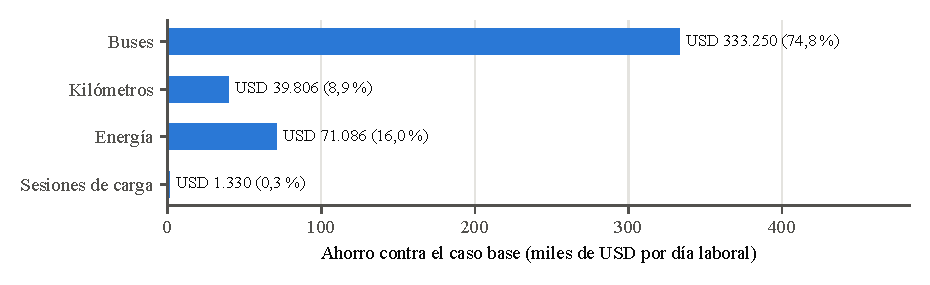
\includegraphics[width=\textwidth]{figures/ahorro_componentes.pdf}
\caption{Ahorro diario del plan frente al caso base por componente del costo, día laboral.}
\label{fig:ahorro}
\end{figure}

\section{Uso de los electroterminales y de la energía}
\label{sec:uso-e}

La Figura~\ref{fig:uso-e} muestra cuántos buses cargan a la vez durante el día laboral en toda la red. El caso base concentra la carga al anochecer y llega a \PicoCargandoBase{} buses cargando a la vez en El Conquistador a las \HoraPicoCargandoBase, con \ElectroterminalesLlenosBase{} electroterminales con todas sus conexiones ocupadas. El plan, en cambio, nunca pasa de \PicoCargandoPlan{} buses cargando a la vez en un electroterminal, entre el \PctConexionesMinPlan{} y el \PctConexionesMaxPlan\,\% de sus conexiones, con el máximo entre las \HoraPicoMinPlan{} y las \HoraPicoMaxPlan. Durante el día los cargadores no son un cuello de botella. El sábado el uso sube, y en \PctConexionesMaxEPlanSabado{} llega al \PctConexionesMaxPlanSabado\,\% de las conexiones.

\begin{figure}[htbp]
\centering
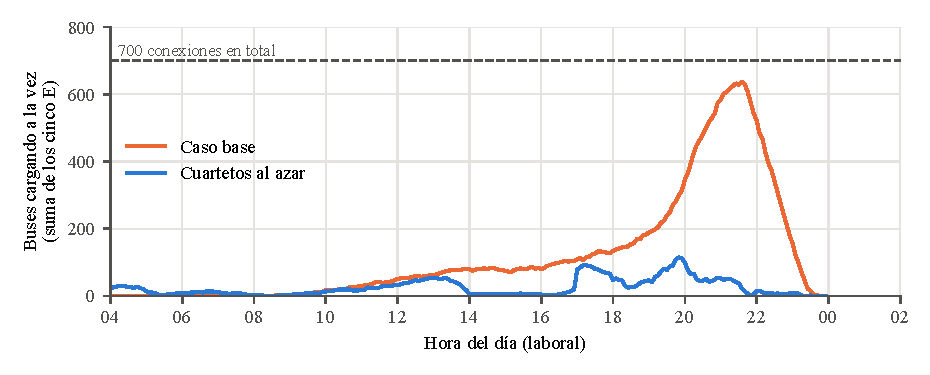
\includegraphics[width=\textwidth]{figures/uso_electroterminales.pdf}
\caption{Buses cargando a la vez en los cinco electroterminales, día laboral.}
\label{fig:uso-e}
\end{figure}

El plan carga muy poca energía durante el día. Los buses parten llenos, la mayoría alcanza a terminar su jornada sin cargar y la energía cargada es \BajaEnergiaCargadaLaboral\,\% menor que en el caso base, apenas el \PctEnergiaCargadaPlanLaboral\,\% de la que se consume. Por eso la energía pesa solo el \PctEnergiaPlanLaboral\,\% del costo del plan. La Figura~\ref{fig:energia-hora} muestra en qué horario se carga, que fue una de las preguntas de la Entrega~2. La mitad de la energía del plan, el \PctEnergiaPuntaPlan\,\%, cae en los tramos de tarifa más alta, contra el \PctEnergiaPuntaBase\,\% del caso base, y la hora en que más carga el plan es de \HoraMasCargaPlan{} a \HoraMasCargaFinPlan{} horas. El plan carga lo justo para terminar sus corridas y lo hace cuando los buses lo necesitan, y en promedio paga USD~\PrecioMedioKwhPlanLaboral{} por kWh, contra \PrecioMedioKwhBaseLaboral{} del caso base. Mover esa carga a horas más baratas casi no cambiaría el costo total, como confirma la sensibilidad a la tarifa (sección~\ref{sec:sens-capacidad}).

\begin{figure}[htbp]
\centering
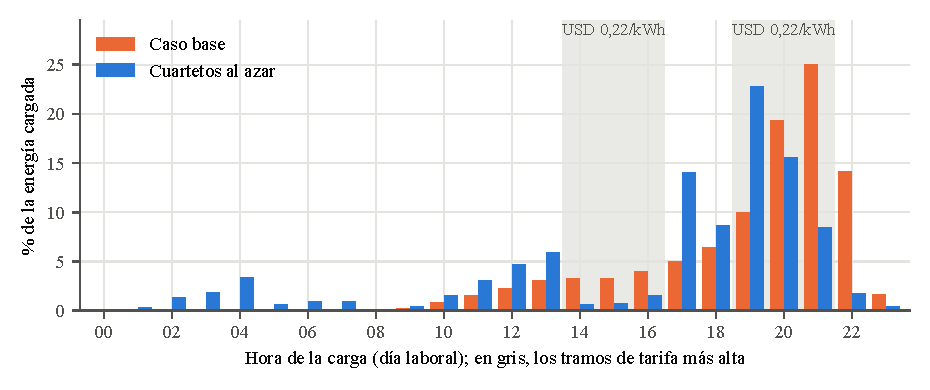
\includegraphics[width=\textwidth]{figures/energia_hora.pdf}
\caption{Distribución horaria de la energía cargada en el día laboral, como porcentaje de lo que carga cada plan.}
\label{fig:energia-hora}
\end{figure}

Las plazas tampoco limitan durante la operación. En el día laboral la ocupación máxima va del \PctPlazasOperacionMin{} al \PctPlazasOperacionMax\,\% de las plazas de cada electroterminal. Se llenan solo al cierre, cuando \BusesTerminanEPlanLaboral{} buses del plan terminan el día estacionados en los electroterminales, y pasada la medianoche permanecen completos entre \MinutosPlazasLlenasMin{} y \MinutosPlazasLlenasMax{} minutos. Ese uso de las plazas al cierre importa para la recarga nocturna, que se analiza en la sección~\ref{sec:repetibilidad}.

La Tabla~\ref{tab:sectores} muestra el plan por sector. El ahorro es parejo, entre 14 y 17\,\% de los buses en cada sector, así que ningún sector concentra la ganancia. Lo que no es parejo es dónde se carga. Los sectores cargan entre el \PctCargaPropiaOtrosMin{} y el \PctCargaPropiaOtrosMax\,\% de su energía en su propio electroterminal, salvo Los Espinos, que carga solo el \PctCargaPropiaTres\,\% en el suyo y el \PctEspinosEnDos\,\% en El Conquistador. Que sus buses puedan cargar donde les queda más a mano es una ventaja de no atar la carga al sector.

\begin{table}[htbp]
\centering
\caption{Plan del día laboral por sector.}
\label{tab:sectores}
\small
\begin{tabular}{@{}lrrrrrr@{}}
\toprule
Sector & Rutas & Corridas & Buses caso base & Buses plan & $\Delta$ buses (\%) & Carga en su E (\%) \\
\midrule
\tabla{sectores}
\bottomrule
\end{tabular}
\fuente{\texttt{09-entrega3/kpi/resultados/kpi\_por\_sector.csv}, plan de cuartetos con semilla 1.}
\end{table}

\section{Elección del método}
\label{sec:metodo-elegido}

La Tabla~\ref{tab:metodos} compara todas las variantes de la mejora en el día laboral con 10, 20 y 40 minutos de búsqueda. La regla fue quedarse con la más barata a igual tiempo, y cuartetos al azar gana con los tres tiempos. La Figura~\ref{fig:tamano} resume el efecto del tamaño del grupo. Con tres buses por grupo cada propuesta es barata, pero hay pocas formas de repartir las corridas; con ocho hay muchas, pero cada intento tarda tanto que en el mismo tiempo se prueban muy pocos. Cuatro buses queda en el punto intermedio de ese dilema \cite{ahuja_vlsn_2002}. La segunda lectura es que elegir los buses al azar le gana a elegirlos por horarios parecidos con cualquier tamaño de grupo. Los grupos parecidos se repiten, la búsqueda queda atrapada en las mismas combinaciones y deja de mejorar antes de agotar el tiempo, como pasa con cuartetos parecidos, que se queda en \BusesMetodoCuartetosParecidos{} buses.

\begin{table}[htbp]
\centering
\caption{Buses del plan del día laboral según la variante de la mejora y el tiempo de búsqueda. Las variantes al azar son el promedio de tres semillas.}
\label{tab:metodos}
\small
\begin{tabular}{@{}lrrrrr@{}}
\toprule
 & \multicolumn{3}{c}{Buses según tiempo de búsqueda} & Costo (USD/día) & \\
\cmidrule(lr){2-4}
Variante & 10 min & 20 min & 40 min & con 40 min & Semillas \\
\midrule
\tabla{metodos_red}
\bottomrule
\end{tabular}
\fuente{\texttt{09-entrega3/octetos/resultados/red\_completa\_417\_L.csv}.}
\end{table}

\begin{figure}[htbp]
\centering
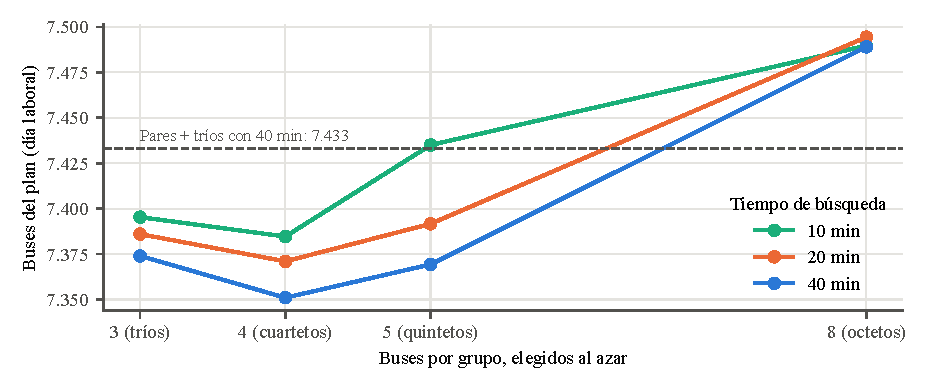
\includegraphics[width=\textwidth]{figures/tamano_grupo.pdf}
\caption{Buses del plan del día laboral según el número de buses por grupo, con selección al azar y tres tiempos de búsqueda.}
\label{fig:tamano}
\end{figure}

\section{Variabilidad de la búsqueda}
\label{sec:variabilidad}

La búsqueda depende de la semilla que fija el sorteo de los grupos. Con \MinutosFinal{} minutos, las tres semillas del día laboral dan entre \BusesSemillaMinLaboral{} y \BusesSemillaMaxLaboral{} buses, entre \BusesSemillaMinSabado{} y \BusesSemillaMaxSabado{} el sábado y entre \BusesSemillaMinDomingo{} y \BusesSemillaMaxDomingo{} el domingo. Con 20 minutos el costo de las tres semillas varía \RuidoSemillas\,\%. Esa dispersión es pequeña frente al ahorro contra el caso base, pero no frente a algunos efectos de la sensibilidad, y por eso se usa como banda de ruido en el capítulo~\ref{ch:sensibilidad}. La búsqueda también depende del reloj y del equipo, de modo que todos los métodos se compararon con el mismo tiempo y en el mismo computador.

\section{Calidad de la solución}
\label{sec:calidad}

El método no garantiza el óptimo, así que su calidad se midió de tres maneras.

La primera usa \CasosChicos{} casos chicos de 2 a 4 rutas, con \CorridasChicosMin{} a \CorridasChicosMax{} corridas, que el modelo exacto resolvió con óptimo demostrado en \MinutosExactaMin{} a \MinutosExactaMax{} minutos cada uno. La Tabla~\ref{tab:brecha-chicos} muestra la brecha de cada variante con \SegundosChicos{} segundos de búsqueda. El plan inicial queda en promedio a \BrechaInicial\,\% del óptimo, pares y tríos a \BrechaParesTrios\,\% y cuartetos al azar a \BrechaCuartetos\,\%, con un peor caso de \BrechaPeorCuartetos\,\%.

\begin{table}[htbp]
\centering
\caption{Brecha al óptimo en los cinco casos chicos, con 120 segundos de búsqueda. Las variantes al azar promedian tres semillas por caso, y el peor caso es la peor corrida individual.}
\label{tab:brecha-chicos}
\small
\begin{tabular}{@{}lrr@{}}
\toprule
Variante & Brecha media (\%) & Peor caso (\%) \\
\midrule
\tabla{brecha_chicos}
\bottomrule
\end{tabular}
\fuente{\texttt{09-entrega3/octetos/resultados/casos\_chicos.csv} y \texttt{casos\_chicos\_exacta.csv}.}
\end{table}

La segunda usa casos medianos, de 6 a 12 rutas, que se resolvieron con el modelo podado (Tabla~\ref{tab:casos-rutas}). Con 5 minutos y una semilla, cuartetos queda a menos de 1\,\% del óptimo en tres de los cuatro casos con óptimo, incluido el de \CorridasRutasDiez{} corridas, donde usa los mismos \BusesOptRutasDiez{} buses del óptimo. En el caso de 8 rutas queda a \BrechaCuartetosRutasOchoAbs\,\% con \BusesCuartetosRutasOcho{} buses contra \BusesOptRutasOcho{}, y ahí pares y tríos lo hace mejor. Ningún tamaño de grupo gana en todos los casos, y la brecha no crece con el número de corridas. En el caso de 12 rutas el modelo exacto se interrumpió a los 34 minutos y no hay óptimo.

\begin{table}[htbp]
\centering
\caption{Casos medianos con la batería del enunciado. Óptimo en buses y USD por día; las heurísticas usan 5 minutos y una semilla y se expresan en \% sobre el óptimo, con sus buses entre paréntesis. En 12 rutas el porcentaje es contra el plan inicial.}
\label{tab:casos-rutas}
\small
\begin{tabular}{@{}lrlrrr@{}}
\toprule
Caso & Corridas & Óptimo & Plan inicial & Pares + tríos & Cuartetos \\
\midrule
\tabla{casos_rutas}
\bottomrule
\end{tabular}
\fuente{\texttt{09-entrega3/octetos/resultados/casos\_rutas*.csv} y \texttt{casos\_medianos*.csv}.}
\end{table}

La tercera obliga a recargar. Con la batería de \Bateria~kWh casi ningún bus de estos casos necesita cargar, de modo que los casos anteriores prueban poco la parte de recarga del método. En las copias con baterías de 150 y 120~kWh (Tabla~\ref{tab:recarga-forzada}) la mejor heurística reduce el costo del plan inicial entre \MejoraRecargaMinCientoCincuenta{} y \MejoraRecargaMaxCientoCincuenta\,\% con 150~kWh y entre \MejoraRecargaMinCientoVeinte{} y \MejoraRecargaMaxCientoVeinte\,\% con 120~kWh. Con recarga, el exacto ya no demuestra el óptimo en 15 minutos, y su mejor plan queda entre \BrechaCotaRecargaMinCientoCincuenta{} y \BrechaCotaRecargaMaxCientoCincuenta\,\% sobre su propia cota. Contra ese mejor plan, que no es el óptimo, la heurística queda en promedio un \DifMediaRecargaCientoCincuentaAbs\,\% más cara con 150~kWh y un \DifMediaRecargaCientoVeinteAbs\,\% con 120~kWh, casi siempre por uno a cuatro buses más. En el caso más grande, de \CorridasGrande{} corridas, la heurística encuentra un plan con \BusesHeurGrande{} buses y USD~\CostoHeurGrande, mejor que el que encontró el exacto en una hora (\BusesExactaGrande{} buses y USD~\CostoExactaGrande). Darle 15 minutos a la heurística en vez de 2 casi no cambia el resultado, porque la búsqueda se detiene sola al no encontrar mejoras. El límite está en las operaciones que prueba y no en el tiempo, y la extensión natural es un movimiento que traspase recargas entre buses.

\begin{table}[htbp]
\centering
\caption{Recarga forzada. Mejor plan del exacto en 15 minutos (una hora en 10 rutas) y mejor heurística con 2 o 15 minutos.}
\label{tab:recarga-forzada}
\footnotesize
\resizebox{\textwidth}{!}{%
\begin{tabular}{@{}rlrrlrlr@{}}
\toprule
 & & & Buses plan & Exacto & Exacto sobre & Heurística & Heurística \\
kWh & Caso & Corridas & inicial & (buses · USD) & su cota (\%) & (buses · USD) & vs exacto (\%) \\
\midrule
\tabla{recarga_forzada}
\bottomrule
\end{tabular}}
\fuente{\texttt{09-entrega3/octetos/resultados/recarga\_bat150*.csv} y \texttt{recarga\_bat120*.csv}.}
\end{table}

En la red completa no hay óptimo, pero sí una cota. Ningún plan puede usar menos buses que las \SimultaneidadLaboral{} corridas en curso a la vez a las \HoraSimultaneidadLaboral{} ni recorrer menos que los kilómetros de servicio, lo que da un piso de USD~\CotaCosto{} al día. El plan queda \BrechaCotaCosto\,\% sobre ese piso en costo y \BrechaCotaBuses\,\% en buses. Es una cota débil, porque ignora la batería, los traslados en vacío y los sectores, de modo que la distancia real al óptimo es menor que esa cifra, aunque no se sabe cuánto.

Con estas tres mediciones la conclusión es que la solución es aproximada y no óptima. En los casos donde el óptimo se puede calcular queda en general a menos de 1\,\%, pero puede llegar a cerca de 5\,\% en algunos casos y con recarga forzada, y en la red completa solo se puede acotar.

\section{Relación con los objetivos}
\label{sec:relacion-objetivos}

El objetivo era un plan factible para toda la red y los tres tipos de día al menor costo posible, y se cumplió en sus tres partes. El plan cubre todas las corridas y pasó el auditor, y reduce el costo frente a una referencia razonable en los tres días. La reducción viene de lo que se esperaba atacar, el tamaño de la flota, y la calidad de la solución quedó medida contra el óptimo. Los dos aprendizajes que no se anticiparon al comenzar son que la mayor parte del ahorro la entrega una buena construcción y no la búsqueda, y que durante el día la infraestructura de carga sobra mientras que de noche falta, que es el tema del capítulo siguiente.


\chapter[SENSIBILIDAD, INCERTIDUMBRE Y REPETIBILIDAD]{Sensibilidad, incertidumbre y repetibilidad} \label{ch:sensibilidad}
% Capítulo 9. Sensibilidad, incertidumbre y repetibilidad (rúbrica 40 pts).

\section{Qué parámetros se sensibilizan y por qué}
\label{sec:justificacion-sens}

Los parámetros se eligieron a partir de los supuestos de la Tabla~\ref{tab:supuestos} y de las preguntas que RED tendría que responder antes de adoptar el plan. Se agrupan en tres familias.

La primera es la capacidad de carga. Las plazas y conexiones son la infraestructura que RED puede ampliar o perder, y el límite eléctrico es un supuesto porque el dato del transformador no existe. Por eso se probaron plazas y conexiones con 20\,\% menos y con 20 y 50\,\% más, la mitad de las conexiones con las mismas plazas, el cierre de cada electroterminal por separado, que mide la resiliencia frente a una falla, y las plazas repartidas según las corridas de cada sector, a propósito del desbalance que preguntó el profesor. Junto con ellas se probó la tarifa de punta un 50\,\% más cara, para ver si el plan mueve su carga de horario.

La segunda es el bus. La batería y el consumo deciden cuántas corridas alcanza a hacer cada bus, y el consumo de \Consumo~kWh/km es un supuesto derivado de la autonomía nominal que ignora la pendiente, el clima y la carga de pasajeros. Se probaron baterías de 300 y 250~kWh, que representan buses distintos o baterías degradadas, y un consumo 10 y 20\,\% mayor.

La tercera son los precios. El costo por bus y por kilómetro vienen del enunciado y no necesariamente son costos reales, así que se variaron en 20\,\% hacia arriba y hacia abajo, y además se agregó el costo de espera que el modelo no cobra.

Cada escenario de capacidad, tarifa y bus se corrió con el plan inicial y con cuartetos al azar, una semilla y 20 minutos, y se compara con una base corrida en la misma tanda, en el mismo computador y con cuatro corridas en paralelo. Los escenarios de precios se evaluaron sobre los mismos planes, sin volver a optimizar. Como con 20 minutos las tres semillas de la base difieren en \RuidoSemillas\,\% de costo, un cambio menor a unos 0,15\,\% no se puede atribuir al escenario. El plan inicial no tiene azar y sirve para confirmar la dirección de cada efecto. %literal

\section{Capacidad de carga y tarifa}
\label{sec:sens-capacidad}

La Tabla~\ref{tab:sensibilidad} y la Figura~\ref{fig:sensibilidad} muestran el resultado. Lo único que mueve el costo es cerrar un electroterminal, y depende de cuál. Cerrar El Conquistador cambia la flota en \SensBusesCierreDos{} buses y el costo en \SensCostoCierreDos\,\%, y cerrar La Reina, en \SensBusesCierreCuatro{} buses y \SensCostoCierreCuatro\,\%. Cerrar Vespucio Norte tiene un efecto intermedio, y cerrar Santa Rosa o Los Espinos queda dentro del ruido. El plan inicial confirma el mismo orden. Aun en el peor cierre el aumento es menor a 1\,\%, porque los buses del sector afectado pueden cargar en otro electroterminal y, como casi no cargan durante el día, el desvío pesa poco.

\begin{table}[htbp]
\centering
\caption{Sensibilidad a la capacidad de carga y a la tarifa, día laboral. Cambios contra la base de la misma tanda (\BusesSensBase{} buses y USD~\CostoSensBase{} con cuartetos, \BusesInicialLaboral{} buses en el plan inicial).}
\label{tab:sensibilidad}
\small
\begin{tabular}{@{}lrrrrr@{}}
\toprule
 & \multicolumn{3}{c}{Cuartetos al azar (20 min)} & \multicolumn{2}{c}{Plan inicial} \\
\cmidrule(lr){2-4}\cmidrule(lr){5-6}
Escenario & Buses & $\Delta$ buses & $\Delta$ costo (\%) & $\Delta$ buses & $\Delta$ costo (\%) \\
\midrule
\tabla{sensibilidad}
\bottomrule
\end{tabular}
\fuente{\texttt{09-entrega3/sensibilidad/resultados/tabla\_sensibilidad.csv}.}
\end{table}

\begin{figure}[htbp]
\centering
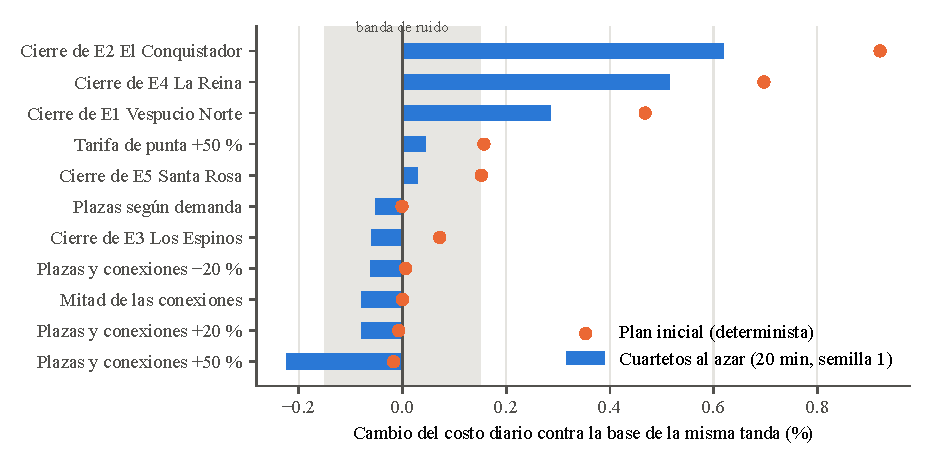
\includegraphics[width=\textwidth]{figures/sensibilidad.pdf}
\caption{Cambio del costo diario en cada escenario de capacidad y tarifa. La franja gris es el ruido entre semillas de la búsqueda.}
\label{fig:sensibilidad}
\end{figure}

Las plazas y las conexiones no limitan la flota en el día aislado, entre 20\,\% menos y 50\,\% más. Con la mitad de las conexiones el plan inicial sale idéntico, lo que coincide con que durante el día se usa como máximo cerca de un quinto de ellas (sección~\ref{sec:uso-e}). Con 50\,\% más de plazas la flota de cuartetos cambia en \SensBusesPlazasMasCincuenta{} buses, pero eso está en el borde del ruido y el plan inicial no se mueve, así que para afirmarlo harían falta más semillas. La tarifa de punta más cara sube el costo del plan inicial en USD~\SensUsdInicialTarifaPunta{} al día (\SensCostoInicialTarifaPunta\,\%), y con cuartetos la diferencia queda dentro del ruido, porque la energía es una fracción mínima del costo.

\section{El bus}
\label{sec:sens-bus}

El bus mismo pesa mucho más que la infraestructura (Tabla~\ref{tab:fisicos}). Con una batería de 250~kWh la flota cambia en \FisDeltaBusesBatDoscientosCincuenta\,\%, y con 20\,\% más de consumo, en \FisDeltaBusesConsumoVeinte\,\%. Con menos autonomía cada bus alcanza a hacer menos corridas antes de tener que cargar, y la carga pasa a ocupar huecos que antes servían para encadenar. La pregunta relevante, sin embargo, es si el ahorro frente al caso base se mantiene, y para responderla el caso base se corrió con la misma batería y el mismo consumo de cada escenario. El caso base también crece, y el ahorro de costo del método queda entre \FisAhorroMin{} y \FisAhorroMax\,\%, prácticamente igual al de la base de la tanda.

\begin{table}[htbp]
\centering
\caption{Sensibilidad a la batería y al consumo, día laboral. Cuartetos al azar con 20 minutos y una semilla; el caso base usa la misma batería y el mismo consumo de cada escenario.}
\label{tab:fisicos}
\footnotesize
\resizebox{\textwidth}{!}{%
\begin{tabular}{@{}lrrrrrrr@{}}
\toprule
 & Batería & Consumo & Buses & Buses & $\Delta$ buses & $\Delta$ costo & Ahorro vs \\
Escenario & (kWh) & (kWh/km) & caso base & plan & plan (\%) & plan (\%) & caso base (\%) \\
\midrule
\tabla{fisicos}
\bottomrule
\end{tabular}}
\fuente{\texttt{09-entrega3/sensibilidad/resultados/fisicos\_417\_L.csv} y \texttt{ahorro\_fisicos.csv}.}
\end{table}

\section{Precios}
\label{sec:sens-precios}

Con el costo por bus o por kilómetro un 20\,\% más alto o más bajo, el ahorro del día laboral queda entre \CostosAhorroMin{} y \CostosAhorroMax\,\% (Tabla~\ref{tab:costos}). Encarecer los buses aumenta un poco el ahorro, porque el método ahorra sobre todo buses, y encarecer los kilómetros lo reduce un poco. Cobrar la espera entre corridas, a USD~\CostoEsperaMinuto{} por minuto, suma cerca del \PctEspera\,\% al costo de ambos planes y deja el ahorro en \AhorroConEspera\,\%. Estos escenarios no se reoptimizaron, de modo que muestran el ahorro de los mismos planes con otros precios.

\begin{table}[htbp]
\centering
\caption{Ahorro de costo del plan frente al caso base con otros precios, sin volver a optimizar (\%).}
\label{tab:costos}
\small
\begin{tabular}{@{}lrrr@{}}
\toprule
Escenario & Laboral & Sábado & Domingo \\
\midrule
\tabla{costos}
\bottomrule
\end{tabular}
\fuente{\texttt{09-entrega3/sensibilidad/resultados/costos\_evaluados.csv} y \texttt{09-entrega3/kpi/resultados/costo\_espera.csv}.}
\end{table}

\section{Incertidumbre en los tiempos de viaje}
\label{sec:incertidumbre}

Los planes se construyen con los tiempos nominales del GTFS, pero en la operación hay congestión. Para medir qué tan frágil es cada plan se simuló su día laboral con tiempos aleatorios, multiplicando la duración de cada corrida y de cada traslado por un factor lognormal de media uno, con coeficientes de variación de 10, 20 y 30\,\% y \ReplicasAtrasos{} réplicas por nivel, usando los mismos números aleatorios para ambos planes. En la simulación un bus nunca sale antes de su horario, de modo que si llega tarde el atraso se arrastra, y el cargador queda reservado hasta la hora programada, así que un bus que llega tarde carga menos. No hay despachadores ni buses de reserva.

\begin{table}[htbp]
\centering
\caption{Simulación de atrasos en el día laboral, promedio de \ReplicasAtrasos{} réplicas.}
\label{tab:atrasos}
\footnotesize
\begin{tabular}{@{}rrrrrrrrr@{}}
\toprule
 & \multicolumn{2}{c}{Corridas con más} & \multicolumn{2}{c}{Atraso percentil} & \multicolumn{2}{c}{Buses bajo} & \multicolumn{2}{c}{Buses sin} \\
 & \multicolumn{2}{c}{de 5 min de atraso (\%)} & \multicolumn{2}{c}{95 (min)} & \multicolumn{2}{c}{la reserva} & \multicolumn{2}{c}{energía} \\
\cmidrule(lr){2-3}\cmidrule(lr){4-5}\cmidrule(lr){6-7}\cmidrule(lr){8-9}
Variación (\%) & Base & Plan & Base & Plan & Base & Plan & Base & Plan \\
\midrule
\tabla{atrasos}
\bottomrule
\end{tabular}
\fuente{\texttt{09-entrega3/incertidumbre/resultados/atrasos.csv}.}
\end{table}

El plan es más frágil que el caso base (Tabla~\ref{tab:atrasos} y Figura~\ref{fig:atrasos}). Con una variación de 10\,\%, el \AtrasadasPlanDiez\,\% de sus corridas sale con más de cinco minutos de atraso, contra el \AtrasadasBaseDiez\,\% del caso base, y \BajoReservaPlanDiez{} buses bajan de la reserva, contra \BajoReservaBaseDiez{}. La explicación está en lo que el método optimiza. Usa menos buses, de modo que hay menos tiempo libre entre corridas para absorber atrasos, y carga solo la energía necesaria, de modo que si un atraso acorta una carga el bus termina bajo la reserva. El caso base, que carga siempre al 100\,\%, tiene un colchón de energía que el plan no tiene. Antes de operar el plan hay que darle holgura, con un margen de energía sobre la reserva en el MILP de recargas, tiempo de colchón antes de cada carga o algunos buses de reserva. Esa holgura le restará parte del ahorro, y cuánto queda por medir. La simulación además supone atrasos independientes, cuando en la realidad la congestión afecta a muchas corridas a la vez, así que los resultados reales podrían ser peores.

\begin{figure}[htbp]
\centering
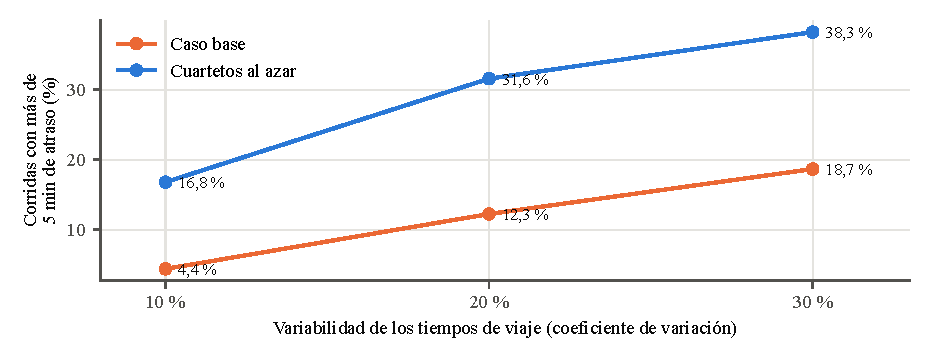
\includegraphics[width=\textwidth]{figures/atrasos.pdf}
\caption{Corridas con más de cinco minutos de atraso según la variabilidad de los tiempos de viaje, día laboral.}
\label{fig:atrasos}
\end{figure}

\section{Repetibilidad del día siguiente}
\label{sec:repetibilidad}

El enunciado fija que todos los buses parten el día con la batería llena, y ambos planes lo cumplen. Pero en la Entrega~2 el equipo docente preguntó cómo se cubre el día siguiente. En el plan los buses terminan el día laboral con \EnergiaFinalPlanLaboral~kWh en promedio, contra \EnergiaFinalBaseLaboral{} en el caso base, porque cargan muy poco durante la operación. Para volver a partir llenos hay que reponer \ReponerMwhLaboral~MWh durante la noche.

Para saber si eso es posible se supuso que cada bus carga en el electroterminal de su sector durante su ventana nocturna, que va de su última llegada a su primera salida del día siguiente, y que todas las conexiones trabajan a \Potencia~kW durante toda la ventana. La Tabla~\ref{tab:repetibilidad} muestra el resultado. En día laboral la ventana mediana dura \VentanaMedianaLaboral{} horas y en ella las \ConexionesTotales{} conexiones alcanzan a entregar solo el \PctCubiertoLaboral\,\% de la energía necesaria. Para reponerla toda harían falta \MwNecesariosLaboral~MW en vez de los \MwInstalados{} instalados, o \ConexionesNecesariasLaboral{} conexiones. El problema es general, aunque desigual. La Reina cubre el menor porcentaje (\ReposPeorPct\,\%) y a Santa Rosa le faltan más conexiones (\ReposMasFaltan), mientras que Vespucio Norte cubre el \ReposMejorPct\,\%. El sábado y el domingo, con menos buses y ventanas más largas, se cubre el \PctCubiertoSabado{} y el \PctCubiertoDomingo\,\%.

\begin{table}[htbp]
\centering
\caption{Recarga nocturna necesaria para repetir el día, por tipo de día.}
\label{tab:repetibilidad}
\footnotesize
\begin{tabular}{@{}lrrrrrrr@{}}
\toprule
 & Energía a & Ventana & \multicolumn{2}{c}{Se alcanza a reponer (\%)} & MW & Conexiones & Conexiones \\
\cmidrule(lr){4-5}
Día & reponer (MWh) & mediana (h) & Plan & Caso base & necesarios & necesarias & faltantes \\
\midrule
\tabla{repetibilidad}
\bottomrule
\end{tabular}
\fuente{\texttt{09-entrega3/kpi/resultados/repetibilidad.csv}. Hay \ConexionesTotales{} conexiones y \MwInstalados~MW instalados.}
\end{table}

El caso base tampoco se repite, ya que en día laboral alcanza a reponer el \PctCubiertoBaseLaboral\,\% y le faltan \ConexionesFaltantesBaseLaboral{} conexiones, de modo que el problema está en la infraestructura frente a una flota eléctrica de este tamaño. El plan sí agrava el problema, porque deja más energía por reponer (\ReponerMwhLaboral{} contra \ReponerBaseMwhLaboral~MWh) y parte de su ahorro en energía corresponde a carga que se traslada a la noche. Si a cada plan se le cobra la energía de esa noche, a la tarifa nocturna y con o sin el costo de sesión, el ahorro del día laboral baja de \BajaCostoLaboral{} a entre \AhorroNocheMinLaboral{} y \AhorroNocheMaxLaboral\,\%, y el semanal de \BajaSemana{} a entre \AhorroNocheMinSemana{} y \AhorroNocheMaxSemana\,\%. Casi todo el ahorro se mantiene porque viene de los buses. Estas cifras son una cota optimista, porque no cuentan el traslado hasta el electroterminal, y \BusesTerminanFueraLaboral{} de los \BusesPlanLaboral{} buses terminan el día en terminales sin cargadores.

\section{Implicancias y robustez de las conclusiones}
\label{sec:implicancias}

La conclusión principal, que el plan cubre el mismo servicio con cerca de 15\,\% menos buses y 14\,\% menos costo, resiste todos los escenarios probados. Ni los precios, ni la capacidad de carga, ni el bus la cambian de signo o de orden de magnitud, y aun cobrando la recarga nocturna el ahorro supera el 12\,\%. Para RED esto tiene tres implicancias prácticas. Ampliar plazas o conexiones no reduce la flota en la operación diurna, de modo que esa inversión solo se justifica por la noche. Los electroterminales que más importan en caso de falla son El Conquistador y La Reina, y conviene asegurar su continuidad de servicio. Y la elección del bus, en batería y consumo, pesa más en la flota que cualquier decisión de infraestructura.

Lo que no resiste igual de bien es la operación con atrasos. El plan funciona en el modelo, pero en la calle necesita holgura, y esa es la principal condición para implementarlo (capítulo~\ref{ch:piloto}).

\section{Limitaciones}
\label{sec:limitaciones}

El modelo tiene límites que conviene declarar. Trata un día aislado y no exige terminar con energía, lo que se compensa solo en parte con el análisis de repetibilidad. Supone carga lineal, cuando las baterías reales cargan más lento cerca del 100\,\%, aunque el plan carga poco y rara vez llega a ese tramo. La velocidad en vacío de \VelocidadVacio~km/h, la potencia y el estado de carga inicial no se variaron. Tampoco se modelan conductores, mantenciones ni la capacidad de los terminales comunes. Los sectores fijos impiden combinar corridas de sectores vecinos, y en la red completa la calidad del plan solo se conoce a través de una cota débil.

\section{Extensiones y mejoras}
\label{sec:extensiones}

El análisis sugiere cinco mejoras. Agregar holgura de energía y de tiempo al MILP de recargas, que es la condición para operar el plan, y modelar la noche exigiendo que la energía final permita repetir el día con la capacidad nocturna de cada electroterminal. Probar un movimiento que traspase recargas entre buses, que es lo que limitó la búsqueda con recarga forzada, y grupos con buses de sectores vecinos. Y agregar capacidad a los terminales comunes y una cota más fuerte para la red, por ejemplo con generación de columnas dentro de un sector.


\chapter[IMPLEMENTACIÓN, PILOTO Y EXTENSIONES]{Implementación, piloto y extensiones} \label{ch:piloto}
% Capítulo 10. Implementación, piloto y extensiones (rúbrica, parte de sensibilidad y extensiones).

Un plan que ahorra más de mil buses en el papel no se puede llevar de golpe a toda la red. Hay que comprobar que funciona con tiempos de viaje reales, conductores reales y la carga nocturna que hoy existe, y hacerlo de modo que un error no afecte el servicio. Este capítulo propone cómo hacerlo por etapas y cómo decidir si el piloto justifica el despliegue.

\section{Antes del piloto}
\label{sec:antes-piloto}

El primer paso es ajustar el método a la operación real, estimando tiempos de viaje por tramo y hora con datos de posicionamiento de los buses, el consumo real con datos de carga, y la capacidad de los terminales de espera y el límite eléctrico de cada electroterminal. Con eso se agrega al MILP de recargas un margen de energía sobre la reserva y un tiempo de colchón antes de cada carga, y se vuelve a correr la simulación de atrasos hasta que el plan con holgura se atrase como máximo lo mismo que el caso base.

\section{Etapas de la implementación}
\label{sec:etapas}

La implementación se propone en tres etapas. En la primera el plan corre en paralelo, sin operarse, durante cuatro a seis semanas en un sector. Cada día se calcula el plan con las corridas del día siguiente y se compara con lo que efectivamente se operó, en buses usados, kilómetros, energía y en qué corridas el plan habría fallado por atrasos o por falta de batería.

En la segunda etapa el plan se opera en un sector piloto, con otro sector como control que sigue operando como hoy. Se propone Vespucio Norte como piloto, porque es el sector más chico, con \RutasSectorUno{} rutas y \BusesPlanSectorUno{} buses en el plan del día laboral. Además carga casi todo en su propio electroterminal (\PctCargaPropiaUno\,\%) y es el que mejor alcanza a recargar de noche (\ReposMejorPct\,\%), de modo que el piloto no depende de resolver primero la infraestructura nocturna. Como control se propone Los Espinos, de tamaño comparable (\BusesPlanSectorTres{} buses) y que casi no comparte carga con el piloto, porque sus buses cargan apenas el \PctEspinosEnUno\,\% de su energía en Vespucio Norte y los de Vespucio Norte el \PctVespucioEnTres\,\% en Los Espinos. Así, un cambio en la forma de cargar del piloto no contamina al control. El piloto debería durar entre ocho y doce semanas.

En la tercera etapa, si el piloto cumple los criterios de la sección siguiente, el plan se extiende sector por sector, empezando por los de mejor cobertura nocturna. En paralelo, RED debería evaluar la ampliación de la carga nocturna, porque con la infraestructura actual ningún plan, tampoco el caso base, permite repetir el día laboral (sección~\ref{sec:repetibilidad}).

\section{Cómo medir el éxito del piloto}
\label{sec:exito}

El piloto se evalúa comparando el sector piloto con el de control y con su propio desempeño antes del piloto, de modo que los cambios de demanda o de tráfico que afecten a ambos no se confundan con el efecto del plan. Se proponen cuatro criterios, que deben cumplirse durante varias semanas seguidas para justificar el despliegue.

El primero es el ahorro. El sector piloto debe usar al menos un 10\,\% menos buses que antes para cubrir las mismas corridas, con un costo por corrida menor que el del control. El método promete cerca de 15\,\% en el modelo, y el margen reconoce que parte del ahorro se gastará en holgura. El segundo es la puntualidad. El porcentaje de corridas con más de cinco minutos de atraso no debe superar al del control en más de un punto porcentual, y no debe haber corridas perdidas por falta de bus. El tercero es la energía. Ningún bus debe quedar bajo la reserva en servicio, y la energía al cierre debe permitir partir el día siguiente con la carga que el plan supone. El cuarto es la operación. Los conductores y despachadores deben poder seguir el plan sin cambios manuales frecuentes, lo que se mide con el número de reasignaciones hechas en el día.

Si se cumple el ahorro pero no la puntualidad, la respuesta es más holgura. Si ocurre lo contrario, conviene revisar si los tiempos de viaje reales dejan menos huecos para encadenar que los del GTFS.

\section{Riesgos de la implementación}
\label{sec:riesgos}

El riesgo principal es operativo. Un plan con menos buses deja menos margen para fallas mecánicas o accidentes, y por eso se recomienda mantener algunos buses de reserva por sector, cuyo costo se puede comparar con el ahorro. El segundo riesgo es la carga nocturna, que limita cuántos sectores se pueden pasar al plan sin ampliar infraestructura. El tercero es que los buses dejan de estar asociados a una ruta, lo que cambia la asignación de conductores y turnos, algo que este proyecto no modeló.


\chapter[CONCLUSIONES]{Conclusiones} \label{ch:conclusiones}
% Capítulo 11. Conclusiones (rúbrica 25 pts).

\section{Hallazgos}
\label{sec:hallazgos}

El problema de programar la flota eléctrica de RED se pudo resolver para toda la red y los tres tipos de día. El plan obtenido cubre las mismas \CorridasLaboral{} corridas del día laboral que un caso base razonable con \AhorroBusesLaboral{} buses menos (\DeltaPctBusesLaboral\,\%) y un costo \BajaCostoLaboral\,\% menor, y en la semana ahorra cerca de USD~\AhorroSemanaMillones{} millones (\DeltaPctSemana\,\%). Ese era el objetivo que se planteó al comienzo, operar el mismo servicio con menos flota.

El ahorro viene casi todo de los buses, que explican cerca de tres de cada cuatro dólares, y la mayor parte se consigue antes de optimizar. Compartir buses entre las rutas de un sector, cargar solo lo necesario y elegir el bus más cercano ya entrega el \PctAhorroInicial\,\% de la reducción de flota. La búsqueda por grupos agrega el resto, y entre las variantes probadas la mejor fue tomar cuatro buses al azar, que es el punto donde el tamaño del grupo y la cantidad de intentos se equilibran.

Durante el día la infraestructura de carga sobra. Como máximo se usa cerca de un quinto de las conexiones de un electroterminal, las plazas solo se llenan al cierre y ampliar o reducir la capacidad casi no cambia la flota. De noche ocurre lo contrario. Para repetir el día laboral habría que reponer \ReponerGwhLaboral~GWh, y las conexiones actuales solo alcanzan para el \PctCubiertoLaboral\,\% de esa energía. Esa es la restricción que viene para RED, y afecta también al caso base.

La solución es aproximada. En los casos donde el óptimo se pudo demostrar queda en promedio a \BrechaCuartetos\,\% de él, en un caso mediano llega a \BrechaCuartetosRutasOchoAbs\,\%, y cuando se obliga a recargar queda cerca de un \DifMediaRecargaCientoCincuentaAbs\,\% sobre el mejor plan que encontró el modelo exacto, al que en el caso más grande supera. En la red completa solo se puede acotar, y queda \BrechaCotaCosto\,\% sobre una cota débil.

\section{Fortalezas y limitaciones}
\label{sec:fortalezas}

La principal fortaleza del trabajo es que el método escala a la red completa sin perder control sobre la factibilidad. Cada plan pasa por un auditor independiente, la búsqueda solo acepta cambios factibles y más baratos, y las cifras del informe se generan desde los resultados, de modo que se pueden rastrear y repetir. La segunda es que la calidad del método se midió con el modelo exacto en casos chicos y medianos. La tercera es que la conclusión principal resiste los cambios de precios, de capacidad de carga y del bus, y aun cobrando la recarga nocturna el ahorro supera el 12\,\%.

Las limitaciones más importantes son dos. El plan es más sensible a los atrasos que el caso base, porque tiene menos buses y carga lo justo, y con tiempos de viaje 10\,\% variables el \AtrasadasPlanDiez\,\% de sus corridas sale atrasado más de cinco minutos. Y el modelo trata cada día por separado, sin exigir que la energía al cierre permita repetirlo. A eso se suman los sectores fijos, que dejan fuera combinaciones entre sectores vecinos, los supuestos sobre la velocidad en vacío y la carga lineal, la ausencia de conductores y mantenciones en el modelo, y una cota débil para la red completa. Mirando hacia atrás, habría convenido incorporar antes la noche y la holgura al modelo en lugar de medirlas al final.

\section{Pasos siguientes}
\label{sec:pasos}

El paso más urgente es agregar holgura de energía y de tiempo al MILP de recargas y medir cuánto ahorro se pierde con ella, porque sin eso el plan no se puede operar. Le siguen modelar la noche y ampliar las operaciones de la búsqueda. Con esas mejoras, la recomendación para RED es un piloto en el sector de Vespucio Norte, primero en paralelo y luego operado frente a un sector de control, con criterios de éxito definidos de antemano en buses, puntualidad y energía, y una evaluación de la ampliación de la carga nocturna antes de extender el plan a toda la red.


\cleardoublepage
\phantomsection \label{references}
\bibliographystyle{apacite}
\renewcommand{\bibname}{REFERENCIAS}
\bibliography{referencias}

\appendix

\newpage
\section[Notación y glosario]{Notación y glosario} \label{an:notacion}
Este anexo reúne las siglas y los símbolos que se usan en el informe. Los términos del problema se definen en la sección~\ref{sec:terminos}.

\begin{table}[H]
\centering
\caption{Siglas.}
\label{tab:siglas}
\small
\begin{tabularx}{\textwidth}{@{}l X@{}}
\toprule
Sigla & Significado \\
\midrule
RED & Red Metropolitana de Movilidad de Santiago \\
GTFS & \emph{General Transit Feed Specification}, formato estándar de horarios de transporte público \\
E-VSP & Programación de vehículos eléctricos (\emph{electric vehicle scheduling problem}) \\
MILP & Programación lineal entera mixta (\emph{mixed-integer linear programming}) \\
KPI & Indicador de desempeño (\emph{key performance indicator}) \\
E1 a E5 & Electroterminales Vespucio Norte, El Conquistador, Los Espinos, La Reina y Santa Rosa \\
T01 a T04 & Terminales comunes, sin cargadores \\
L, S, D & Día laboral, sábado y domingo \\
\bottomrule
\end{tabularx}
\end{table}

\begin{table}[H]
\centering
\caption{Símbolos del modelo del capítulo~\ref{ch:modelo}.}
\label{tab:simbolos}
\small
\begin{tabularx}{\textwidth}{@{}l X@{}}
\toprule
Símbolo & Significado \\
\midrule
\(N\) & Corridas del tipo de día \\
\(T,\ E,\ F\) & Terminales comunes, electroterminales y lugares de término (\(F=T\cup E\)) \\
\(s_i,\ f_i,\ L_i,\ \sigma(i)\) & Inicio, término, distancia de servicio y sector de la corrida \(i\) \\
\(A\) & Pares de corridas que un bus puede encadenar directo \\
\(K_{ij},\ R\) & Opciones de carga entre \(i\) y \(j\), y conjunto de todas ellas \\
\(e(k),\ a_k,\ h_k,\ g_k,\ p_k\) & Electroterminal, km de ida y de vuelta, energía máxima y precio medio de la opción \(k\) \\
\(d_{ij},\ d^{0}_i,\ d^{1}_{i\ell}\) & Km del traslado entre corridas, desde el terminal de salida y hasta el lugar de término \\
\(B,\ m,\ r\) & Batería, reserva y consumo por km \\
\(c^{B},\ c^{D},\ c^{S}\) & Costo por bus, por km y por sesión \\
\(P_e,\ C_e\) & Plazas y conexiones del electroterminal \(e\) \\
\(\Omega,\ \alpha_{k\omega}\) & Bloques de cinco minutos e indicador de que la opción \(k\) carga en el bloque \(\omega\) \\
\(u_i,\ z_{i\ell}\) & La corrida \(i\) inicia una jornada, o la termina en \(\ell\) \\
\(x_{ij},\ y_{ijk},\ q_{ijk}\) & Encadenamiento directo, encadenamiento con carga y kWh cargados \\
\(e_i\) & Energía del bus al terminar la corrida \(i\) \\
\bottomrule
\end{tabularx}
\end{table}


\newpage
\section[Correcciones atendidas]{Correcciones atendidas de las entregas anteriores} \label{an:correcciones}
Este anexo lista los comentarios recibidos en las entregas anteriores y dónde se atendió cada uno en este informe.

\begin{table}[H]
\centering
\caption{Comentarios de la corrección del informe 2.}
\label{tab:corr-informe2}
\footnotesize
\begin{tabularx}{\textwidth}{@{}X p{5.2cm}@{}}
\toprule
Comentario & Dónde se atiende \\
\midrule
Cómo afecta que los terminales comunes tengan capacidad ilimitada y qué pasa con una capacidad realista & Se midió la ocupación máxima de cada terminal en ambos planes, sección~\ref{sec:supuestos} \\
Si se va a escalar y cuánto cuesta hacerlo & El método se aplicó a la red completa en los tres tipos de día, capítulo~\ref{ch:resultados} \\
Falta justificar mejor la metodología seleccionada & Revisión por familias y justificación, secciones~\ref{sec:familias} y~\ref{sec:justificacion} \\
Hacer un diagrama de la metodología y del caso base, con entradas y salidas, y ponerlo antes & Figura~\ref{fig:enfoque} en el capítulo~\ref{ch:problema} y Figura~\ref{fig:flujo} \\
Qué tan bueno o malo es programar primero y cargar después, y si hay estudios & Sección~\ref{sec:evolucion}, con literatura y la evidencia propia \\
Confunde que se diga que aumentan los buses al incorporar la electricidad como si fuera una decisión & La batería se presenta como restricción, secciones~\ref{sec:descripcion} y~\ref{sec:evolucion} \\
En qué se basa combinar construcción cronológica y mejora local & Sección~\ref{sec:justificacion} \\
Del costo del caso base, qué es lo más mejorable & Composición del costo, sección~\ref{sec:resultado-caso-base} \\
No se entendía cómo se relacionaba la metodología con el diagnóstico anterior & El capítulo~\ref{ch:literatura} encadena diagnóstico, evolución y método \\
Hacer dibujos de las operaciones & Figura~\ref{fig:operaciones} \\
Para qué es el MILP & Sección~\ref{sec:milp-local} \\
Poner el diagrama de flujo más arriba, sin código & Figura~\ref{fig:flujo}, al inicio del capítulo~\ref{ch:estrategia} \\
\bottomrule
\end{tabularx}
\end{table}

\begin{table}[H]
\centering
\caption{Comentarios de la presentación de la Entrega 2 que siguen vigentes.}
\label{tab:corr-presentacion}
\footnotesize
\begin{tabularx}{\textwidth}{@{}X p{5.2cm}@{}}
\toprule
Comentario & Dónde se atiende \\
\midrule
Que el caso base incluya la carga, aunque sea de manera básica & Capítulo~\ref{ch:caso-base} \\
Explicitar los supuestos sobre lo que no está en los datos, como tráfico y mantenciones & Tablas~\ref{tab:preparacion} y~\ref{tab:supuestos} \\
Decir de dónde sale cada porcentaje y cada costo & Notas de fuente en cada tabla y sección~\ref{sec:descripcion} \\
Comparar los indicadores contra el caso base y no contra metas fijas & Sección~\ref{sec:kpis} \\
Justificar la comparación contra una cota que no es factible & Secciones~\ref{sec:kpis} y~\ref{sec:calidad} \\
Definir corrida, traslado en vacío y jornada & Sección~\ref{sec:terminos} \\
Mostrar el peso de cada costo y en qué horario cargan los buses & Tabla~\ref{tab:caso-base}, Figuras~\ref{fig:ahorro} y~\ref{fig:energia-hora} \\
Cómo se cubre el día siguiente & Sección~\ref{sec:repetibilidad} \\
\bottomrule
\end{tabularx}
\end{table}

\begin{table}[H]
\centering
\caption{Comentarios de la corrección del informe 1.}
\label{tab:corr-informe1}
\footnotesize
\begin{tabularx}{\textwidth}{@{}X p{5.2cm}@{}}
\toprule
Comentario & Dónde se atiende \\
\midrule
Definir corrida antes de usarla y distinguirla de recorrido y viaje & Sección~\ref{sec:terminos} \\ %literal
No es necesario discutir la flota declarada, basta decir que la flota es una decisión & Sección~\ref{sec:curva} \\
Explicar las siglas & Primera aparición y anexo~\ref{an:notacion} \\
Presentar el objetivo completo, con electroterminales y horarios & Secciones~\ref{sec:problema-intro} y~\ref{sec:descripcion} \\
Aclarar de qué es la distancia usada para los sectores & Sección~\ref{sec:energia-datos} \\
Aclarar qué significa la energía en MWh de la tabla de escala & Sección~\ref{sec:energia-datos} \\
Mostrar el gráfico de corridas a lo largo del día & Figura~\ref{fig:corridas-dia} \\
Los KPI se comparan contra un caso base y no son valores fijos & Sección~\ref{sec:kpis} \\
Llamar costo total y costo energético a los indicadores de costo, y comparar todos los costos & Sección~\ref{sec:descripcion} y Tabla~\ref{tab:caso-base} \\
Aclarar si corrida y viaje son lo mismo & Se usa solo corrida, sección~\ref{sec:terminos} \\ %literal
Qué son los terminales convencionales & Terminales comunes, secciones~\ref{sec:terminos} y~\ref{sec:energia-datos} \\
Si la carga lineal es un supuesto propio o de la metodología & Tabla~\ref{tab:supuestos} \\
\bottomrule
\end{tabularx}
\end{table}


\newpage
\section[Formulación del MILP local de recargas]{Formulación del MILP local de recargas} \label{an:milp-local}
Este anexo presenta la formulación del MILP local que el método resuelve en cada intento (\texttt{metodo\_hibrido/conjunta.py}). Corresponde a la formulación de la sección 5.5 del informe~2, extendida a grupos de hasta cuatro jornadas.

Sea \(\mathcal{B}\) el conjunto de jornadas de una propuesta, con \(1\le |\mathcal{B}|\le 4\). Para cada bus \(b\in \mathcal{B}\) la búsqueda fija sus corridas y su orden, indexadas por \(I_b=\{1,\dots,n_b\}\), y \(G_b=\{2,\dots,n_b\}\) son los huecos antes de cada corrida. Sean \(A_b\subseteq T\) y \(Z_b\subseteq T\cup E\) los terminales candidatos de inicio y de término. Las ventanas de carga candidatas del hueco \(i\) forman \(K_{bi}\), y \(J=\{(b,i,k)\mid b\in \mathcal{B},\ i\in G_b,\ k\in K_{bi}\}\). Cada ventana fija un electroterminal \(e(k)\), un número \(N_{bik}\) de bloques completos de \MinutosBloque~minutos y una tarifa media \(\bar p_{bik}\). Las distancias \(d^{\mathrm{ini}}_{bt}\), \(d^{\mathrm{fin}}_{bt}\) y \(d_{bi}\) son las del traslado de salida, de regreso y entre corridas, y \(\delta_{bik}=a_{bik}+h_{bik}-d_{bi}\) es el desvío adicional por ir a cargar. La energía máxima por bloque es \(g=\EnergiaBloque\)~kWh.

Las variables son \(x_{bt},z_{bt}\in\{0,1\}\) para el terminal inicial y final, \(y_{bik}\in\{0,1\}\) para usar la ventana \(k\), \(q_{bik}\ge 0\) para la energía cargada y \(E_{bi}\in[m,B]\) para la energía al terminar la corrida \(i\). El modelo minimiza los kilómetros variables, las sesiones y la energía,
\begin{equation}
\min\ c^{D}\sum_{b\in \mathcal{B}}\Bigl(\sum_{t\in A_b}d^{\mathrm{ini}}_{bt}x_{bt}+\sum_{t\in Z_b}d^{\mathrm{fin}}_{bt}z_{bt}+\sum_{i\in G_b}d_{bi}\Bigr)
+\sum_{(b,i,k)\in J}\bigl[(c^{S}+c^{D}\delta_{bik})\,y_{bik}+\bar p_{bik}\,q_{bik}\bigr],
\end{equation}
sujeto a
\begin{align}
\sum_{t\in A_b}x_{bt}=1,\qquad \sum_{t\in Z_b}z_{bt}&=1 && \forall b\in \mathcal{B},\\
E_{b1}&=B-r\Bigl(L_{b1}+\sum_{t\in A_b}d^{\mathrm{ini}}_{bt}x_{bt}\Bigr) && \forall b\in \mathcal{B},\\
\sum_{k\in K_{bi}}y_{bik}\le 1,\qquad 0\le q_{bik}&\le g\,N_{bik}\,y_{bik} && \forall b\in \mathcal{B},\ i\in G_b,\ k\in K_{bi},\\
E_{bi}&=E_{b,i-1}-r\,(d_{bi}+L_{bi})+\sum_{k\in K_{bi}}\bigl(q_{bik}-r\,\delta_{bik}\,y_{bik}\bigr) && \forall b\in \mathcal{B},\ i\in G_b,\\
y_{bik}=1\ \Rightarrow\ E_{b,i-1}-r\,a_{bik}&\ge m,\quad E_{b,i-1}-r\,a_{bik}+q_{bik}\le B && \forall (b,i,k)\in J,\\
E_{b,n_b}-r\sum_{t\in Z_b}d^{\mathrm{fin}}_{bt}z_{bt}&\ge m && \forall b\in \mathcal{B},
\end{align}
y a la capacidad que deja libre el resto del plan. Si \(O_{e\ell}\) y \(H_{e\ell}\) son las plazas y conexiones que ocupan los demás buses en el intervalo \(\ell\) del electroterminal \(e\), y los indicadores \(\alpha\) y \(\beta\) valen uno cuando una ventana o un término ocupan ese intervalo,
\begin{align}
\sum_{(b,i,k)\in J}\alpha_{bik,e\ell}\,y_{bik}+\sum_{b\in \mathcal{B}}\sum_{t\in Z_b}\beta_{bt,e\ell}\,z_{bt}&\le P_e-O_{e\ell},\\
\sum_{(b,i,k)\in J}\alpha_{bik,e\ell}\,y_{bik}&\le C_e-H_{e\ell}.
\end{align}
Antes de resolver se descartan las conexiones y ventanas que no alcanzan en tiempo. El costo por bus no aparece en el modelo, porque cuántos buses hay lo decide la búsqueda al vaciar una jornada. Para comparar propuestas con distinto número de jornadas se suma \(c^{B}|\mathcal{B}|\) y los kilómetros de servicio, y un candidato \(S'\) reemplaza al plan \(S\) solo si el auditor lo aprueba y \(C(S')<C(S)-10^{-5}\).


\newpage
\section[Parámetros y tablas complementarias]{Parámetros del escenario y tablas complementarias} \label{an:parametros}
La Tabla~\ref{tab:parametros} reúne los parámetros del escenario base que usan el caso base, el método y el modelo exacto, con su origen.

\begin{table}[H]
\centering
\caption{Parámetros del escenario base.}
\label{tab:parametros}
\footnotesize
\begin{tabularx}{\textwidth}{@{}p{3.2cm} X p{2.4cm}@{}}
\toprule
Elemento & Valor & Origen \\
\midrule
Corridas & \CorridasLaboral{} laborales, \CorridasSabado{} de sábado y \CorridasDomingo{} de domingo, en \RutasLaboral{} rutas & GTFS, reconstruidas \\
Batería & \Bateria~kWh, llena al inicio del día; reserva de \Reserva~kWh (\PctReserva\,\%) & Enunciado \\
Consumo & \Consumo~kWh/km, igual con y sin pasajeros & Derivado \\
Carga & Hasta \Potencia~kW por conexión, en bloques de \MinutosBloque~min de hasta \EnergiaBloque~kWh, carga parcial & Enunciado \\
Traslados en vacío & Distancias viales dirigidas, a \VelocidadVacio~km/h & Supuesto \\
Costos & USD~\CostoBus{} por bus, USD~\CostoKmUnit{} por km, USD~\CostoSesion{} por sesión, energía de USD~\TarifaMin{} a \TarifaMax{} por kWh según la hora & Enunciado \\
Espera & USD~\CostoEsperaMinuto{} por minuto, fuera del objetivo & Enunciado, evaluada aparte \\
Electroterminales & E1 (\PlazasUno), E2 (\PlazasDos), E3 (\PlazasTres), E4 (\PlazasCuatro) y E5 (\PlazasCinco) plazas, cada una con su conexión; disponibles todo el día & Enunciado \\
Terminales comunes & T01 a T04, sin cargadores y sin límite de plazas; Los Acacios se excluyó porque su dirección no calza entre fuentes & Decisión del grupo \\
Flota & Sin máximo; la flota declarada de \FlotaDeclarada{} buses no se impone & Aclaración docente \\
Sectores & Cinco, de \RutasSectorUno, \RutasSectorDos, \RutasSectorTres, \RutasSectorCuatro{} y \RutasSectorCinco{} rutas; cada bus atiende un solo sector y carga en cualquier electroterminal & Decisión del grupo \\
Búsqueda & Cuartetos al azar, \MinutosFinal{} min por tipo de día, tres semillas; MILP local con dos segundos por intento, tolerancia de 2\,\% y un hilo & Decisión del grupo \\
\bottomrule
\end{tabularx}
\end{table}


\newpage
\section[Reproducción de los resultados]{Reproducción de los resultados} \label{an:reproduccion}
El código, las pruebas y los resultados agregados están en el repositorio público \url{https://github.com/nfariasl/capstone-buses-electricos}. Los datos del curso (\texttt{01-datos}, unos 1,3~GB) y los planes bus por bus no están en el repositorio por su tamaño. Se instalan Python~3.12 y los paquetes con %literal
\begin{verbatim}
python3 -m venv .venv-optimizacion
.venv-optimizacion/bin/pip install "gurobipy>=12,<13" numpy scipy \
    pandas matplotlib pytest
\end{verbatim}
y se necesita una licencia académica de Gurobi, porque la gratuita del paquete no alcanza para grupos de tres buses o más. Con los datos copiados en \texttt{01-datos}, cada resultado se repite con la orden indicada en la Tabla~\ref{tab:reproduccion}. Como la búsqueda se corta por reloj, repetir una corrida en otro computador da un plan parecido pero no idéntico.

\begin{table}[H]
\centering
\caption{Cómo reproducir cada resultado del informe.}
\label{tab:reproduccion}
\footnotesize
\begin{tabularx}{\textwidth}{@{}p{3.4cm} X@{}}
\toprule
Resultado & Orden o script \\
\midrule
Instancias de la red completa & \texttt{metodo\_hibrido/preparar\_completa.py --servicio L} (también S y D) \\
Caso base & \texttt{codigo/tres\_fases/caso\_base.py} \\
Métodos en la red y casos chicos & \texttt{09-entrega3/octetos/correr\_todo.sh} \\
Casos medianos y recarga forzada & \texttt{09-entrega3/octetos/correr\_noche.sh} y \texttt{correr\_rutas\_heuristicas.sh} \\
Indicadores y uso de electroterminales & \texttt{09-entrega3/kpi/kpi\_planes.py}, \texttt{uso\_electroterminales.py} y \texttt{ocupacion\_plazas.py} \\
Repetibilidad y recarga nocturna & \texttt{09-entrega3/kpi/repetibilidad.py} y \texttt{costo\_recarga\_nocturna.py} \\
Terminales comunes & \texttt{09-entrega3/kpi/ocupacion\_terminales.py} \\
Sensibilidad & \texttt{09-entrega3/sensibilidad/correr\_sensibilidad.sh}, \texttt{correr\_fisicos.sh} y \texttt{caso\_base\_fisicos.sh} \\
Atrasos & \texttt{09-entrega3/incertidumbre/simular\_atrasos.py --replicas 20} \\
Cifras, tablas, figuras y PDF de este informe & \texttt{09-entrega3/informe3/compilar.sh} \\
\bottomrule
\end{tabularx}
\end{table}


\newpage
\section[Declaración de uso de IA]{Declaración de uso de IA en este informe y presentación asociada} \label{an:ia}
\noindent Grupo 29

\medskip
\noindent ¿Hicieron uso de herramientas de IA en su trabajo para este informe y/o presentación? \quad SI \underline{\ X\ } \quad NO \underline{\ \ \ }

\medskip
\noindent ¿Cuáles de las siguientes alternativas mejor describe el uso que hicieron de IA (puede ser más de una)?

\begin{itemize}
\item[X] Apoyo a la redacción, ortografía, estructura gramatical, etc., de los documentos.
\item[X] Apoyo al análisis de datos e información asociada al problema.
\item[X] Búsqueda y/o filtro de referencias, contenidos web, literatura, etc., relevante al proyecto.
\item[\ ] Apoyo para el desarrollo de modelos asociados al proyecto.
\item[X] Apoyo en el desarrollo de código computacional necesario para el proyecto.
\item[X] Apoyo en el análisis de resultados (por ejemplo, de distintas corridas computacionales, tendencias de predicciones, etc.).
\item[X] Apoyo para construir figuras, diagramas, etc.
\item[\ ] Apoyo para obtener conclusiones a partir de los análisis de resultados.
\item[\ ] Otro, especificar.
\end{itemize}

\noindent Herramientas usadas. Claude (Anthropic), a través de Claude Code.

\medskip
\noindent Reflexión. La IA fue un apoyo útil, sobre todo para escribir y depurar código, ordenar los resultados de muchas corridas y dar forma a las tablas y figuras. Después de las alucinaciones que detectamos en el informe~1, cada referencia se verificó en su fuente antes de citarla, y cada cifra del informe la genera un script desde los resultados, sin copiarla a mano. El planteamiento del problema, las decisiones de modelación, la elección del método y del caso base, y la interpretación de los resultados las tomó el grupo en sus reuniones y en las conversaciones con el profesor y el ayudante. Todo el código se revisó y se probó antes de usar sus resultados.

\vspace{1.2cm}
\noindent\begin{tabular}{@{}p{0.45\textwidth}p{0.45\textwidth}@{}}
\rule{5.5cm}{0.4pt} & \rule{5.5cm}{0.4pt} \\
Gonzalo Anguita & Diego Barrios \\[1cm]
\rule{5.5cm}{0.4pt} & \rule{5.5cm}{0.4pt} \\
Gustavo Cueto & Nicolás Farías \\[1cm]
\rule{5.5cm}{0.4pt} & \rule{5.5cm}{0.4pt} \\
Fernando González & Ricardo Palma \\[1cm]
\rule{5.5cm}{0.4pt} & \\
Cristóbal Rehbein & \\
\end{tabular}


\end{document}
